\usepackage{here}

\title{Twitterにおけるユーザープロフィールと拡散力の関係分析}
\author{プロジェクトマネジメントコース\\
ソフトウェア開発管理グループ\\
矢吹研究室\\
1142016\\
井上 乃祐}
\date{}
\begin{document}


\definecolor{dkgreen}{rgb}{0,0.6,0}
\definecolor{gray}{rgb}{0.5,0.5,0.5}
\definecolor{mauve}{rgb}{0.58,0,0.82}

\lstset{
language={Python},
basicstyle={\small},
identifierstyle={\small},
commentstyle={\small\itshape\color{dkgreen}},
keywordstyle={\small\bfseries\color{blue}},
ndkeywordstyle={\small},
stringstyle={\small\ttfamily\color{mauve}},
frame={tb},
breaklines=true,
columns=[l]{fullflexible},
numbers=left,
xrightmargin=0zw,
xleftmargin=3zw,
numberstyle={\scriptsize},
stepnumber=1,
numbersep=1zw,
lineskip=-0.5ex
}

\maketitle

%本テンプレートの余白は,卒論マニュアルで指示されたものとは違っているが,1ページあたりの文字数は40文字x40行と,卒論マニュアル通りになっている。文字間隔や行間隔を調整して,余白をマニュアル通りにすることもできるが,それでは文章が読みにくくなるため,このような対応をしている。

%\noindent
□□□□□□□□□■□□□□□□□□□■□□□□□□□□□■□□□□□□□□□■
□□□□□□□□□■□□□□□□□□□■□□□□□□□□□■□□□□□□□□□■
□□□□□□□□□■□□□□□□□□□■□□□□□□□□□■□□□□□□□□□■
□□□□□□□□□■□□□□□□□□□■□□□□□□□□□■□□□□□□□□□■
□□□□□□□□□■□□□□□□□□□■□□□□□□□□□■□□□□□□□□□■
□□□□□□□□□■□□□□□□□□□■□□□□□□□□□■□□□□□□□□□■
□□□□□□□□□■□□□□□□□□□■□□□□□□□□□■□□□□□□□□□■
□□□□□□□□□■□□□□□□□□□■□□□□□□□□□■□□□□□□□□□■
□□□□□□□□□■□□□□□□□□□■□□□□□□□□□■□□□□□□□□□■
□□□□□□□□□■□□□□□□□□□■□□□□□□□□□■□□□□□□□□□■
□□□□□□□□□■□□□□□□□□□■□□□□□□□□□■□□□□□□□□□■
□□□□□□□□□■□□□□□□□□□■□□□□□□□□□■□□□□□□□□□■
□□□□□□□□□■□□□□□□□□□■□□□□□□□□□■□□□□□□□□□■
□□□□□□□□□■□□□□□□□□□■□□□□□□□□□■□□□□□□□□□■
□□□□□□□□□■□□□□□□□□□■□□□□□□□□□■□□□□□□□□□■
□□□□□□□□□■□□□□□□□□□■□□□□□□□□□■□□□□□□□□□■
□□□□□□□□□■□□□□□□□□□■□□□□□□□□□■□□□□□□□□□■
□□□□□□□□□■□□□□□□□□□■□□□□□□□□□■□□□□□□□□□■
□□□□□□□□□■□□□□□□□□□■□□□□□□□□□■□□□□□□□□□■
□□□□□□□□□■□□□□□□□□□■□□□□□□□□□■□□□□□□□□□■
□□□□□□□□□■□□□□□□□□□■□□□□□□□□□■□□□□□□□□□■
□□□□□□□□□■□□□□□□□□□■□□□□□□□□□■□□□□□□□□□■
□□□□□□□□□■□□□□□□□□□■□□□□□□□□□■□□□□□□□□□■
□□□□□□□□□■□□□□□□□□□■□□□□□□□□□■□□□□□□□□□■
□□□□□□□□□■□□□□□□□□□■□□□□□□□□□■□□□□□□□□□■
□□□□□□□□□■□□□□□□□□□■□□□□□□□□□■□□□□□□□□□■
□□□□□□□□□■□□□□□□□□□■□□□□□□□□□■□□□□□□□□□■
□□□□□□□□□■□□□□□□□□□■□□□□□□□□□■□□□□□□□□□■
□□□□□□□□□■□□□□□□□□□■□□□□□□□□□■□□□□□□□□□■
□□□□□□□□□■□□□□□□□□□■□□□□□□□□□■□□□□□□□□□■
□□□□□□□□□■□□□□□□□□□■□□□□□□□□□■□□□□□□□□□■
□□□□□□□□□■□□□□□□□□□■□□□□□□□□□■□□□□□□□□□■
□□□□□□□□□■□□□□□□□□□■□□□□□□□□□■□□□□□□□□□■
□□□□□□□□□■□□□□□□□□□■□□□□□□□□□■□□□□□□□□□■
□□□□□□□□□■□□□□□□□□□■□□□□□□□□□■□□□□□□□□□■
□□□□□□□□□■□□□□□□□□□■□□□□□□□□□■□□□□□□□□□■
□□□□□□□□□■□□□□□□□□□■□□□□□□□□□■□□□□□□□□□■
□□□□□□□□□■□□□□□□□□□■□□□□□□□□□■□□□□□□□□□■
□□□□□□□□□■□□□□□□□□□■□□□□□□□□□■□□□□□□□□□■
■■■■■■■■■■■■■■■■■■■■■■■■■■■■■■■■■■■■■■■■
□□□□□□□□□■□□□□□□□□□■□□□□□□□□□■□□□□□□□□□■%文字数チェック用





\chapter*{謝辞}
本論文作成にあたり,矢吹太朗准教授には長期に渡り熱意のあるご指導,ご鞭撻いただき感謝の言葉もありません.そして,多くの助言をくださいました矢吹研究室の同期,後輩の皆様に感謝いたします.
\tableofcontents%目次

\chapter{序論}

\section{本章の構成}

本章では,本研究の背景・目的について記す

\section{研究背景}
Twitterは2006年に開始したサービスで,コミュニケーションツールのひとつとして利用されているソーシャル・ネットワーキング・サービスである.それは月当たりのアクティブユーザーは全世界で13億5000万人,投稿数は1日当たり約5億ツイートされていると言われ,多くの人に使われている.
その中にリツイートという機能があり,似たような内容でもリツイートされた回数に違いがあることに気付いた.そこで私はユーザープロフィールが拡散力に影響があるのではないかと考えた.


\section{研究目的}
Twitterのリツイートされたデータを収集し,その収集されたデータ(リツイートされたもの)のアイコンをいくつかのタグに分類し,分析することで,Twitterにおけるユーザーのアイコンが拡散力に影響があるかを調べ,情報の本質でないアイコン部分が本質に与える影響を調べる.

\chapter{手法}

\section{本章の構成}
本章では研究方法について記す.

\section{研究方法}

VirtualBoxをインストールして仮想マシンを作成し,そこにUbuntuをインストールする.その後,Ubuntu上でPythonとTweepyをインストールして,Streaming APIを使用するプログラムを実行し,リツイートされたツイートを集める.

その後,リツイートされたツイートのアイコンをいくつかの成分で分類し,Rを用いて重回帰分析をする.



\chapter{Twitterについて}


\section{本章の構成}
本章では本研究で使用するTwitterについて記す.


\section{Twitterとは}

Twitterとはツイートと呼ばれる短文を投稿し,共有するソーシャル・ネットワーキング・サービスである.ツイートは最大140字からなる短文であり,ユーザーからはつぶやきと呼ばれている.そのつぶやきは基本的に全世界の不特定多数のユーザーが閲覧できる.

\begin{figure}[H]
\centering
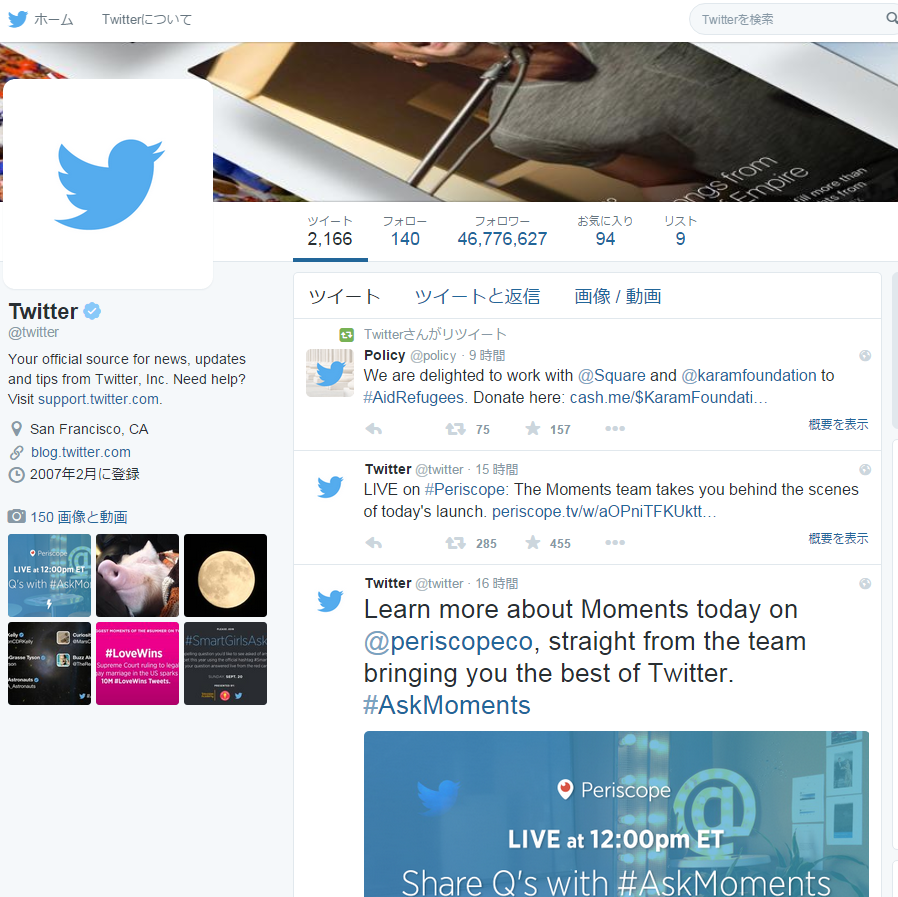
\includegraphics[width=12cm]{twitter000.png}
\caption{Twitterの画面}\label{実際のTwitterの画面}
\end{figure}

\section{用語}
Twitterで使用する用語に関して解説する.

\subsection{ツイート}

140字以下の文字列のことであり,つぶやきと呼ばれる.


\begin{figure}[H]
\centering
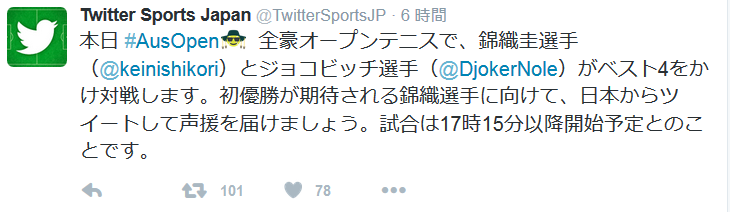
\includegraphics[width=12cm]{tweet001.png}
\caption{ツイート}\label{実際のツイートの画面}
\end{figure}

\subsection{ユーザー}

Twitterを利用している者のことを指す.

\subsection{ユーザー名}

ユーザー名とは半角英数字,アンダーバーから計15文字以内で作る,ユーザーの名前である.

\subsection{タイムライン}

自分のホーム画面の事である.フォローしているユーザーのつぶやき,自分のつぶやきなどの情報が羅列している.
そのタイムラインにリツイートされたツイートも流れてくる.

\begin{figure}[H]
\centering
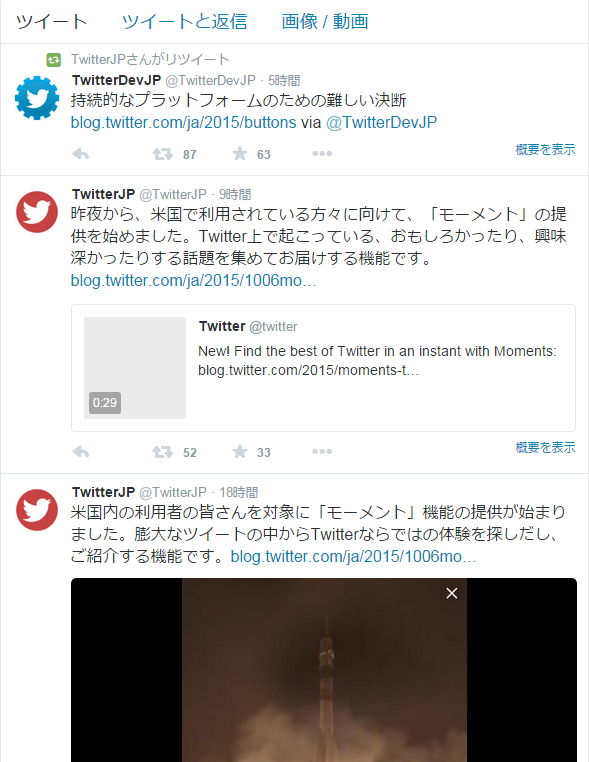
\includegraphics[width=15cm]{twitterTL.png}
\caption{タイムライン}\label{タイムライン}
\end{figure}


\subsection{フォロー}

フォローボタンを押しユーザーをフォローすることによって,自分のタイムラインにそのユーザーのつぶやきが表示されるようにする機能の事である.

\subsection{フォロワー}

自分をフォローしているユーザーの事である.フォロワーのタイムラインには自分(フォローされている人)のつぶやきが表示される.

\subsection{リプライ(返信)}

特定のユーザー名(@...)から始まるツイートをリプライという.そのユーザー宛のツイートということになる.リプライを送った側と,送られた側の両方をフォローしているユーザーのタイムラインには表示されるが,片方のみをフォローしている第三者のタイムラインには表示されない.

\subsection{お気に入り(Favorites)}

あとで読み返したいツイートをお気に入りに入れてTwitter上でログ(記録)化することができる.自分のツイートを含む,全てのツイートに対して有効.発言者がツイートを削除した場合,お気に入りからも削除される.

\subsection{メンション}

特定の「@ユーザー名」を含むツイート.リプライと違って,ツイート内のどこに「@ユーザー名」が入っていてもよい.


\subsection{リツイート}

他の人のツイートを再びツイートするというもの.自分のタイムラインに流れてきたツイートをリツイートすると,自分のフォロワーのタイムラインにそのツイートが流れる.逆に自分がフォローしているユーザーがリツイートすれば,自分のタイムラインにそのツイートが流れる.

\begin{figure}[H]
\centering
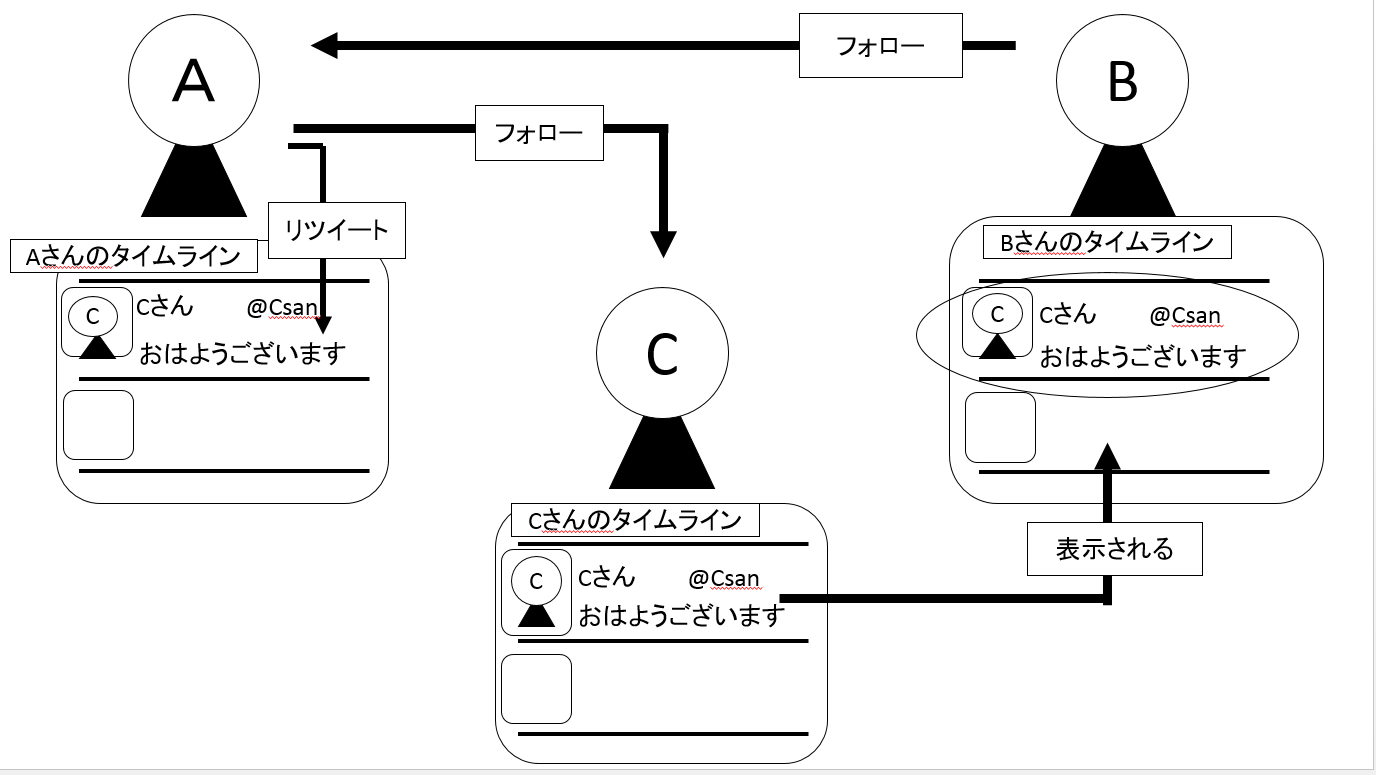
\includegraphics[width=15cm]{rtrogic.png}
\caption{リツイートの仕組み}\label{リツイートの仕組み}
\end{figure}

\section{Twitter APIについて}

本研究で使用するTwitterから情報を取得するためのプログラムとして,Twitter APIを使用する.本章ではTwitter APIに関することを記す.

\subsection{API}

APIとは,Application Programming Interfaceの略で,あるコンピュータプログラム(ソフトウェア)の機能や管理するデータなどを,外部の他のプログラムから呼び出して利用するための手段やデータ形式を定めた規約のこと\cite{api}.
例えば,「Aと言うファイルをBという名前でコピーし,作業完了したらポップアップウィンドウを出して知らせる」というプログラムを作るとしたら,どのような動きをするのかパートに分けてみると以下のようになる.

\begin{enumerate}
 \item Aというファイルを選択.
 \item 実行ボタンを押すと(3)のステップへ.
 \item データをコピーする.
 \item コピーされたデータをBと言う名前をつけ保存.
 \item ポップアップウィンドウを出して作業完了を伝える.
\end{enumerate}

\clearpage

この(1)~(5)の作業を全て1から作成するとかなりの手間が掛かる,それをAPIで作るならば

\begin{enumerate}
 \item ファイルを選択するAPI.
 \item ボタンを押すとプログラムを動かすAPI.
 \item データをコピーするAPI.
 \item ファイルに名前をつけるAPI.
 \item ウィンドウを出してメッセージを出すAPI.
\end{enumerate}
を組み合わせるだけでプログラムができる.

\begin{figure}[H]
\centering
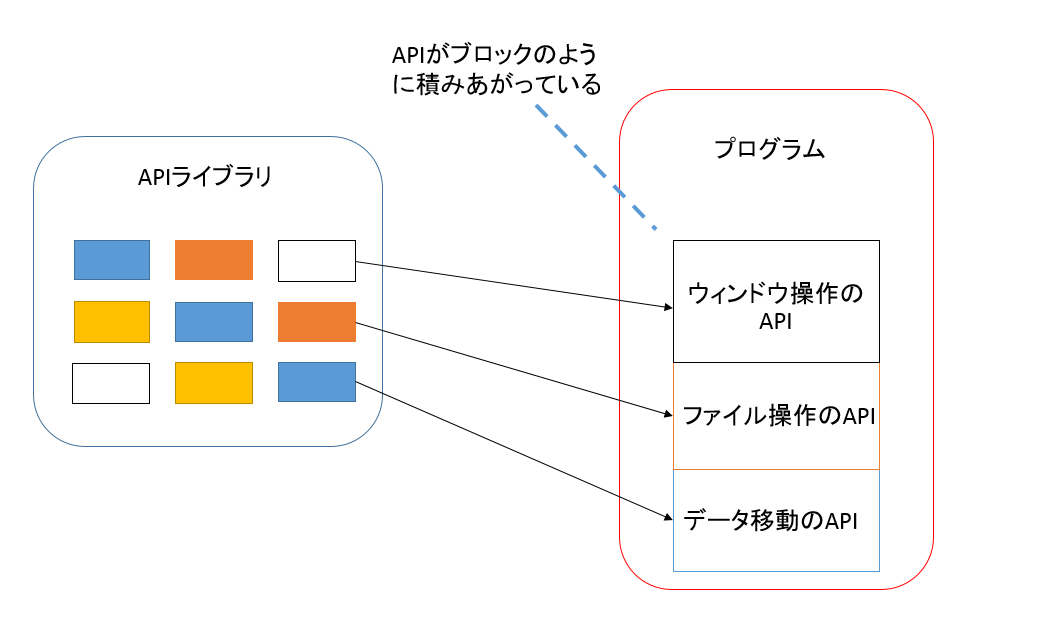
\includegraphics[width=15cm]{API.png}
\caption{APIのイメージ}\label{APIのイメージ}
\end{figure}



\subsection{Twitter API}

Twitter社提供しているサービスで,WebサイトやアプリケーションなどからTwitterの機能を呼び出すことができ,このAPIを利用することでツイートの参照や検索などを行えるアプリケーション開発ができるようになる\cite{twitterapi}.


\subsection{Streaming API}

本研究で使用するAPI.タイムラインの変更をリアルタイムに受け取ることができる.

\subsection{アクセストークン}

アクセストークンとは,Twitterへツイートする際にログインする場合のアカウント情報を記号化してまとめた文字列である.





\section{VirtualBoxとは}
VirtualBoxは,使用しているPC上に仮想的なPCを作成し,別のOSをインストール・実行できるフリーのPC仮想化ソフト.

例えば使用中のパソコンがWindows7とする.PC仮想化ソフトを使うと、そのWindows7上でWindows8やLinuxOSを動作させることがでできる\cite{VirtualBox}.
\begin{figure}[H]
\centering
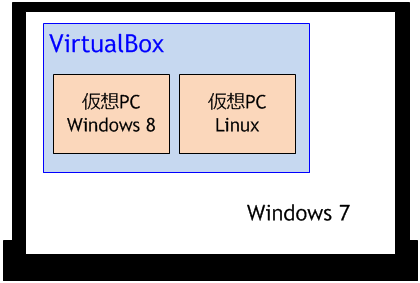
\includegraphics[width=15cm]{virtualbox00.png}
\caption{VirtualBoxのイメージ}\label{VirtualBoxのイメージ}
\end{figure}



\section{用語}

\subsection{OS}

基本となるソフトウェアのこと.OperationSystem(オペレーティング・システム)の略で,直訳すると案内システムとなります.

具体的には,キーボードやマウス・タッチパッドから入力した情報をアプリケーションに伝える役割を果たす,最も基本的なソフトウェアのことです\cite{os}.


\subsection{ホストマシン}

処理能力を持ち,ネットワークを通じて処理やサービスを別のマシンに提供するコンピュータのことである\cite{host}.


\subsection{ホストOS}

ホストOSとは,仮想マシン環境で仮想的なOSを動作させているOSのことである.
LinuxがインストールされているコンピュータでWindowsを操作したり,WindowsでMac OS Xを動作させたりすることができる.仮想コンピュータの使用のため,VirtualBoxが必要となる.

\subsection{仮想マシン}

実際のコンピュータやサーバー上に,VirtualBoxのような仮想化ソフトによって作り出される仮想的なコンピュータを指す.


\subsection{ゲストOS}

ゲストOSとは,ひとつのコンピュータ上で別をコンピュータをエミュレートする「仮想マシン」と呼ばれる環境において,仮想マシン上で動いているOSのことである.

たとえば,「仮想マシン」の環境を用意して,Windows上でLinuxを動かす場合,LinuxがゲストOSとなる.このとき,WindowsはホストOSと呼ばれる.

また,ゲストOSは,仮想マシンの環境からは,アプリケーションとして認識されるため,ゲストOSを動かすには,ホストOSの正常な状態が前提となる.ただし,ゲストOSに以上が生じても,仮想マシン環境そのものには影響はないため,仮想マシン環境を起動させたまま,ゲストOSを再起動させることが可能となっている.なお,仮想マシンを実現するソフトは,VirtualBoxやVMwareなどがある.\cite{guest}



\subsection{仮想ディスク}

ゲストマシンが使用する仮想ハードディスクのことである.仮想ディスクの実体はホストマシン内にファイルとして存在する.

\clearpage


\chapter{Ubuntuについて}

\subsection{本章の構成}
本章では本研究で使用するUbuntuについて記す.
\subsection{Ubuntuとは}

Ubuntu(ウブントゥ) とは,コミュニティ により開発されているオペレーティングシステムです.ラップトップ,デスクトップ,そしてサーバーに利用することができます.Ubuntuには,家庭・学校・職場で必要とされるワープロやメールソフトから,サーバーソフトウェアやプログラミングツールまで,あらゆるソフトウェアが含まれています\cite{Ubuntu}.



\section{プログラムを使用するまでの流れ}

\subsection{VirtualBoxのインストール}

VirtualBoxのダウンロードサイト(http://www.oracle.com/technetwork/server-storage/virtualbox/downloads/index.html?ssSourceSiteId=otnjp)にアクセスし,Platformから自分のOSのインストーラーをダウンロードする.

\begin{figure}[H]
\centering
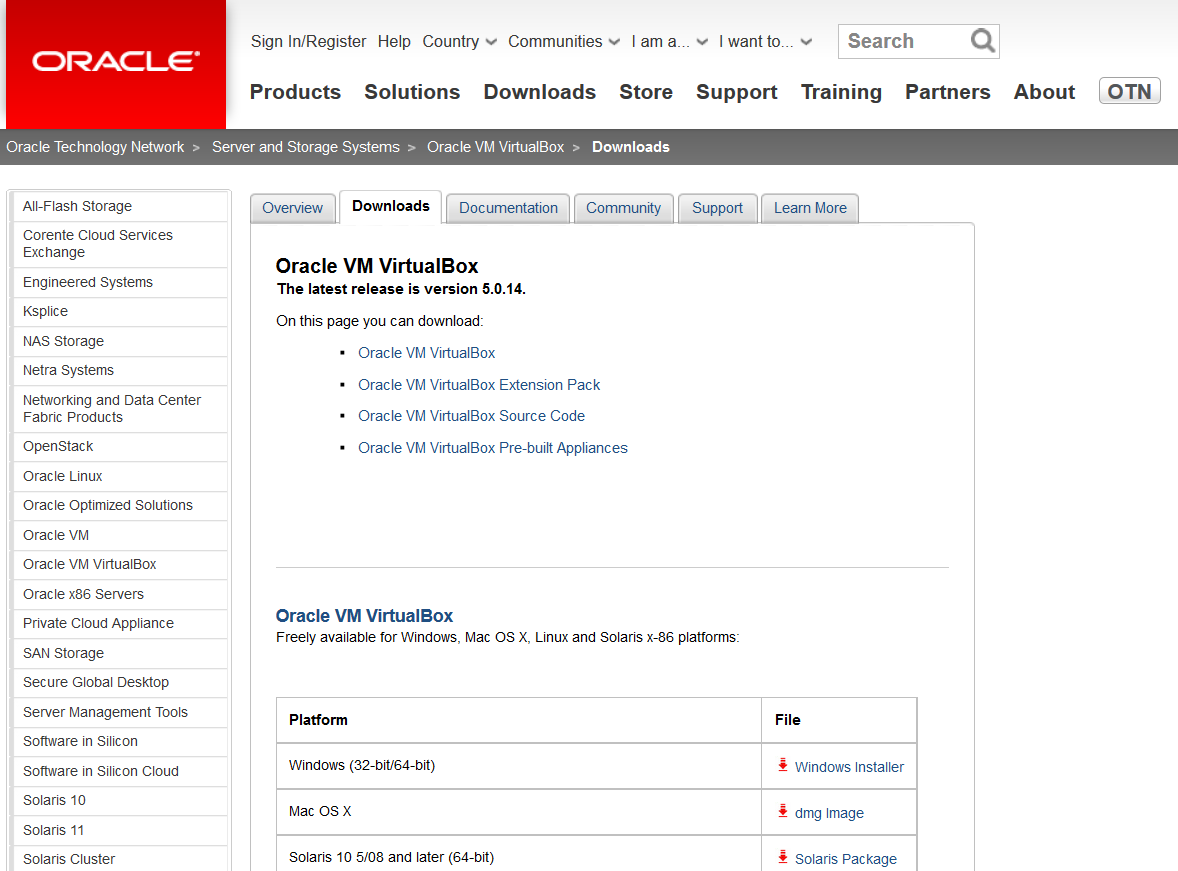
\includegraphics[width=15cm]{virtualbox001.png}
\caption{ダウンロードサイト}\label{virtualboxダウンロードサイトの画像}
\end{figure}
インストーラーを起動し,セットアップウィザードを起動し,指示に従いインストールを開始する.
その後Warning Network Interfacesが表示されたら「Yes」をクリックする.

\begin{figure}[H]
\centering
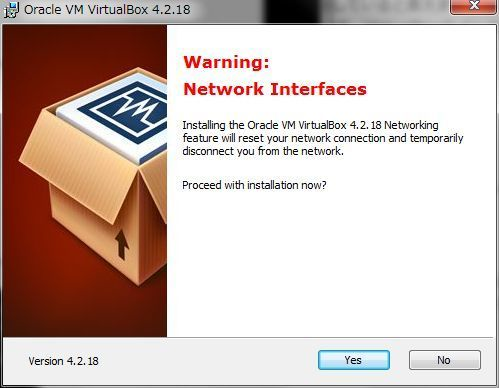
\includegraphics[width=15cm]{virtualbox002.png}
\caption{インストール画面1}\label{virtualboxインストール画面1}
\end{figure}

Ready to Installが表示されたら「Install」をクリックする.
\begin{figure}[H]
\centering
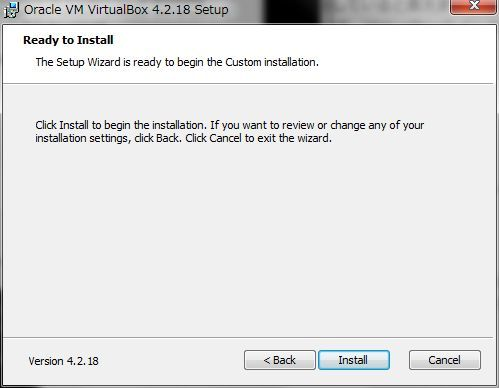
\includegraphics[width=15cm]{virtualbox003.png}
\caption{インストール画面2}\label{virtualboxインストール画面2}
\end{figure}

インストール中にユーザーアカウント制御によってインストールを許可するか否かを聞いてくるが,「はい(Y)」をクリックする.
次に「Windows セキュリティ」ダイアログが表示されたら,「Oracle Corporationからのソフトウエアを常に信頼する(A)」をチェックし,
「インストール(I)」をクリックする.

\begin{figure}[H]
\centering
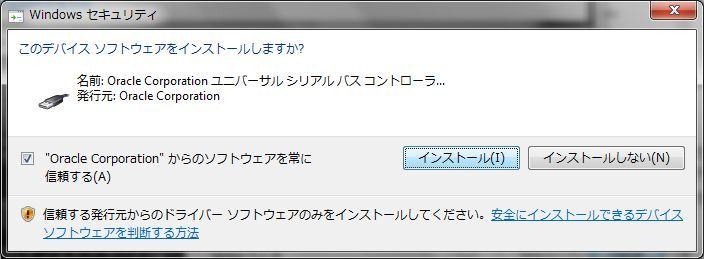
\includegraphics[width=15cm]{virtualbox004.png}
\caption{インストール画面3}\label{virtualboxインストール画面3}
\end{figure}
インストールが終了すると,デスクトップ上にVirtualBoxのショートカットが作成され,インストールが完了する.


\clearpage


\subsection{Ubuntuのインストール}

UbuntuのISOデータを http://www.ubuntulinux.jp/ よりダウンロードする.
先ほどインストールしたVirtualBoxを起動し,仮想マシンの作成をする.

\begin{figure}[H]
\centering
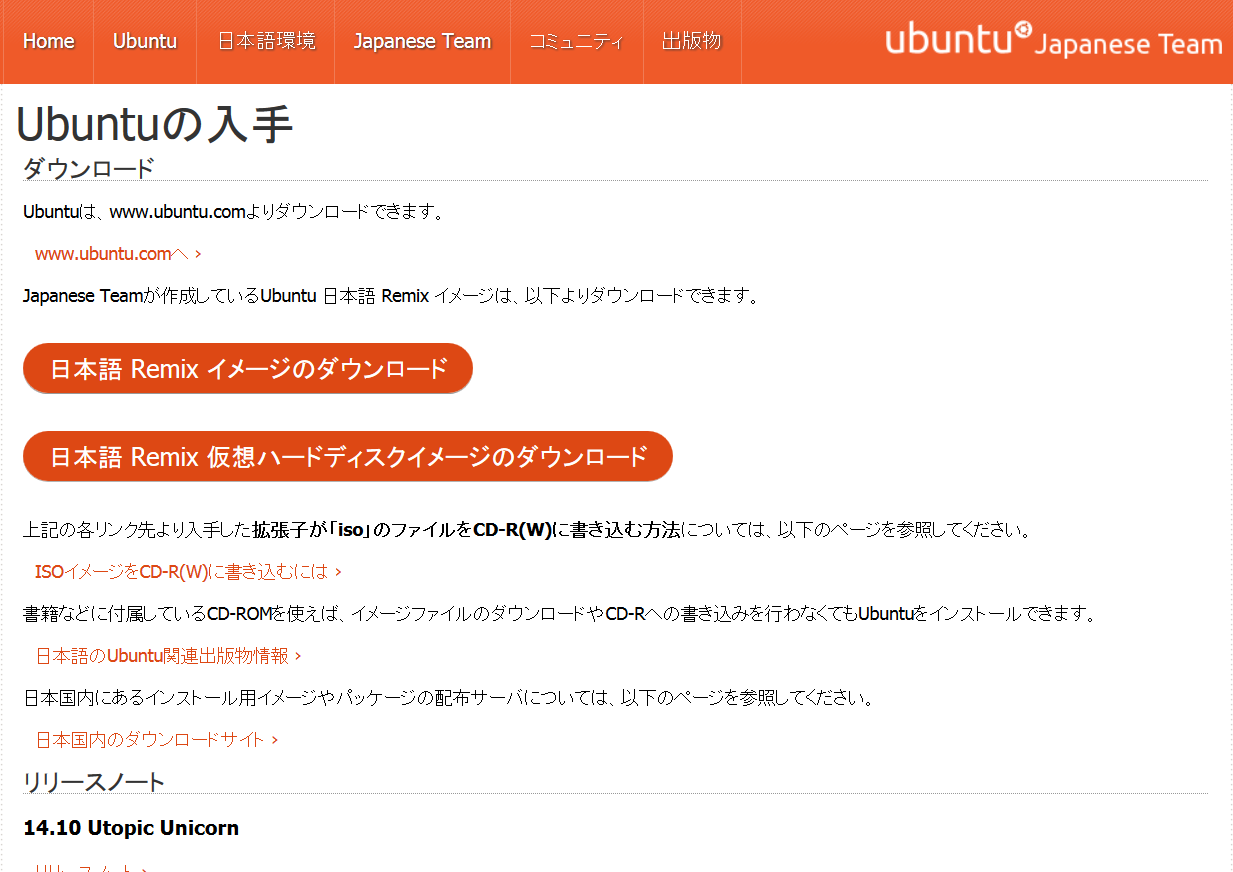
\includegraphics[width=15cm]{ubuntuiso.png}
\caption{Ubuntuのダウンロードページ}\label{Ubuntuのダウンロードページ}
\end{figure}

\subsection{仮想マシンの作成}

デスクトップ上のショートカットからVirtualBoxを起動する.その後VirtualBoxのホーム画面が表示されたら,「新規(N)」をクリックする.その後作成する仮想マシンの名前,メモリサイズ,仮想HDDの設定画面に移動する.

\begin{figure}[H]
\centering
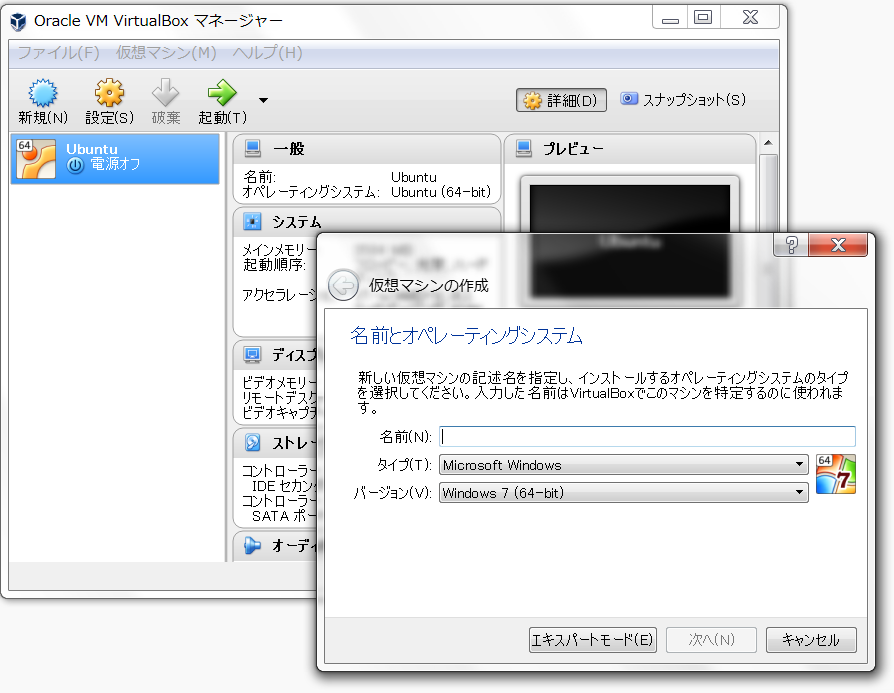
\includegraphics[width=15cm]{vb001.png}
\caption{仮想マシンの名前の設定画面}\label{仮想マシンの設定画面}
\end{figure}

仮想マシンのメモリサイズの設定は以下のように行う.設定後「次へ(N)」をクリックする.

\begin{figure}[H]
\centering
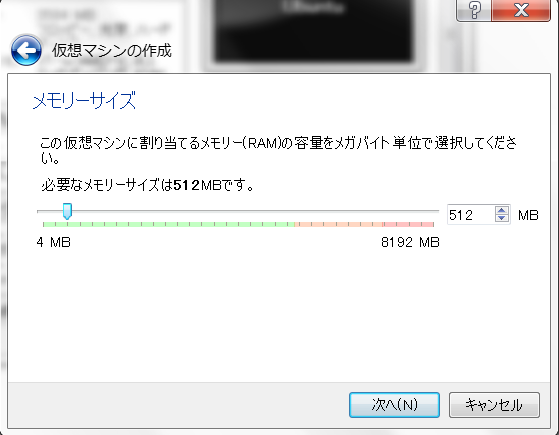
\includegraphics[width=15cm]{vb002.png}
\caption{仮想マシンのメモリサイズ設定画面}\label{仮想マシンの設定画面}
\end{figure}

仮想マシンの仮想HDDのファイルの形式を指定する.


\begin{figure}[H]
\centering
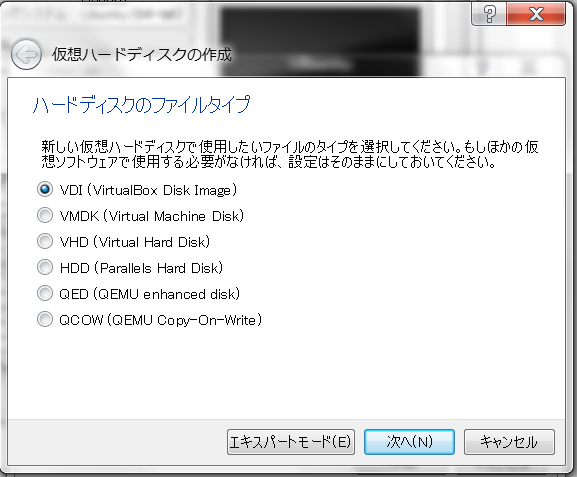
\includegraphics[width=15cm]{vb003.png}
\caption{仮想HDDのファイル形式作成画面}\label{仮想マシンの設定画面}
\end{figure}

作成するハードドライブのファイルの名前を指定する.



\begin{figure}[H]
\centering
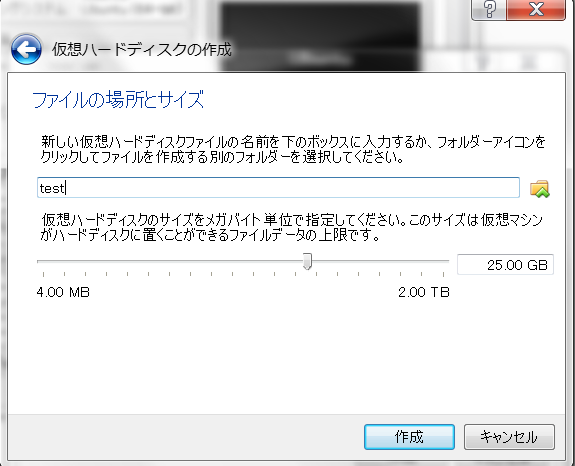
\includegraphics[width=15cm]{vb004.png}
\caption{仮想HDDの作成画面}\label{仮想マシンの設定画面}
\end{figure}

「作成」をクリックしたら以下の画面が表示され,仮想HDDが作成されると自動的にこの画面は閉じられる.


\begin{figure}[H]
\centering
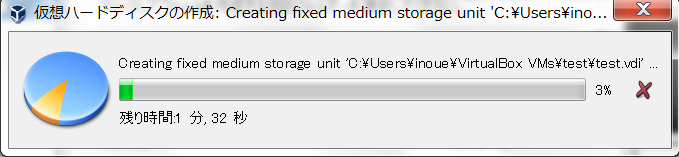
\includegraphics[width=15cm]{vb005.png}
\caption{仮想HDDの作成画面}\label{仮想マシンの設定画面}
\end{figure}

\clearpage


その後先ほど作成した仮想マシンを起動すると,インストール開始画面が表示される.

その後「設定(S)」をクリックし,「ストレージツリー(S)」の項目にある「空」選択する.さらに「属性」内にあるディスクのマークをクリックすると「仮想光学ディスクファイルを選択...」をクリックしUbuntuのISOイメージを選択する.

\begin{figure}[H]
\centering
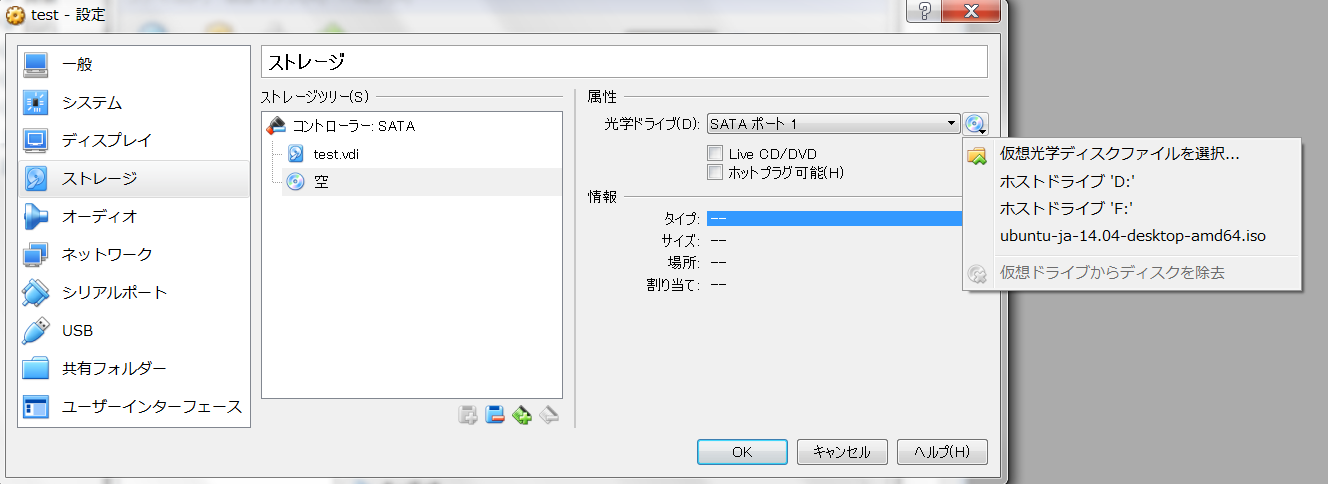
\includegraphics[width=15cm]{vb006.png}
\caption{ISOイメージ設定}\label{仮想マシンの設定画面}
\end{figure}

「OK」をクリックした後,仮想マシンを起動させると以下のような仮想マシン内でのインストールが始まる.

\begin{figure}[H]
\centering
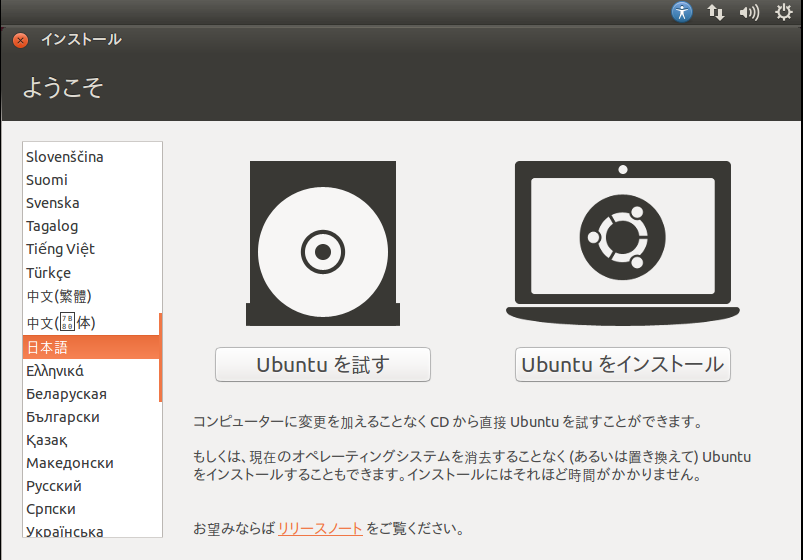
\includegraphics[width=15cm]{ubuntuinstall00.png}
\caption{インストール開始画面}\label{インストール開始画面}
\end{figure}

下の画面が出たら任意で項目にチェックを入れ,「続ける」をクリックする.
\begin{figure}[H]
\centering
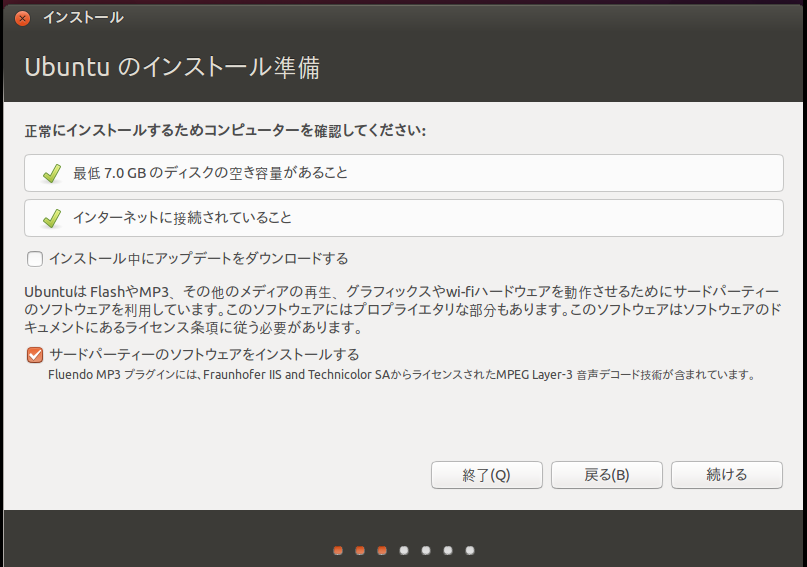
\includegraphics[width=15cm]{ubuntuinstall01.png}
\caption{インストール準備画面}\label{インストール準備画面}
\end{figure}

「Encrypt the new Ubuntu installation for security」,「Use LVM with the new Ubuntu installation」のチェックをはずし,「続ける」をクリックする.

\begin{figure}[H]
\centering
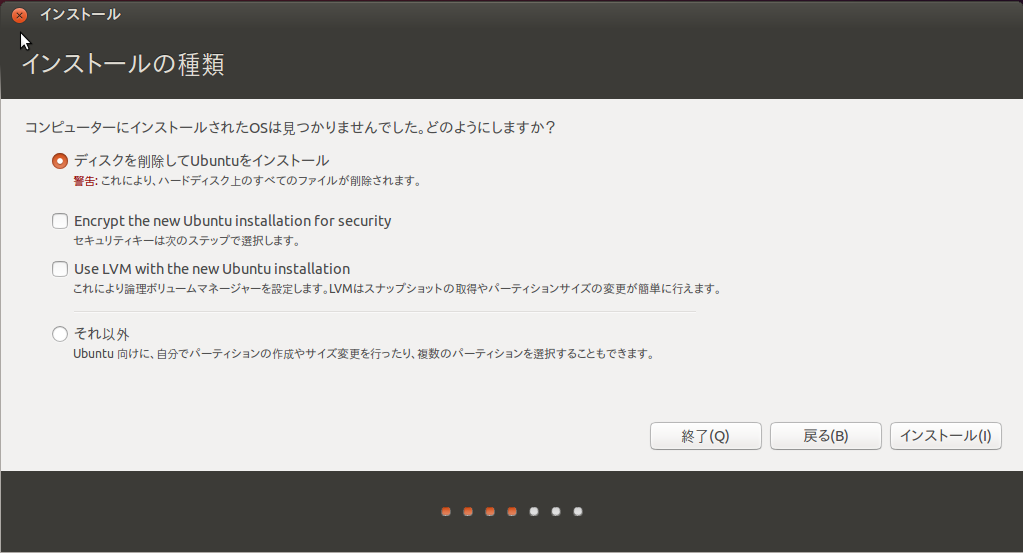
\includegraphics[width=15cm]{ubuntuinstall02.png}
\caption{インストールの種類}\label{インストール準備画面2}
\end{figure}

以下の画面でタイムゾーンを選択する.デフォルトで東京(Tokyo)が選択されているので,「続ける」をクリックする.

\begin{figure}[H]
\centering
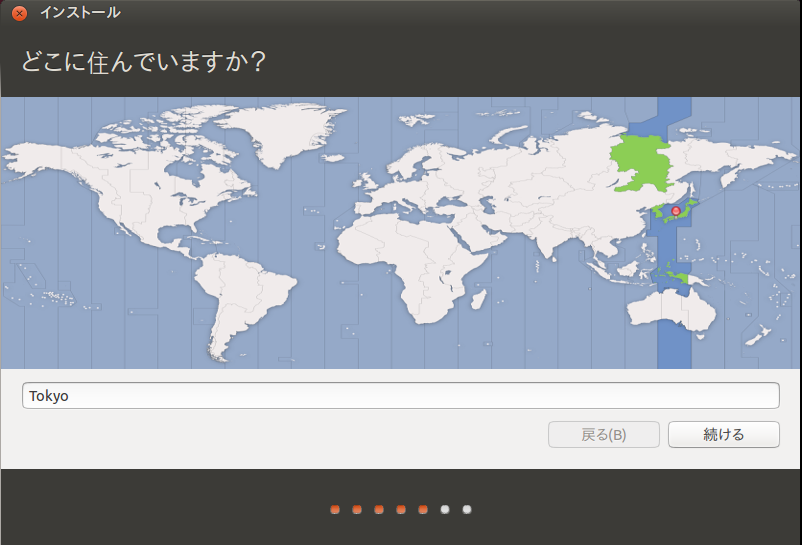
\includegraphics[width=15cm]{ubuntuinstall03.png}
\caption{タイムゾーン}\label{タイムゾーン}
\end{figure}


以下の画面でキーボード配列を選択する.そのまま「続ける」をクリックする.

\begin{figure}[H]
\centering
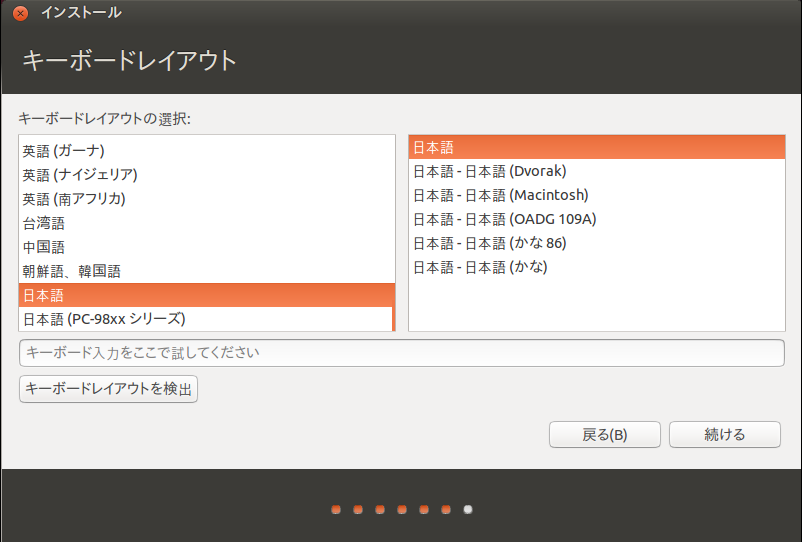
\includegraphics[width=15cm]{ubuntuinstall04.png}
\caption{キーボード配列}\label{キーボード配列}
\end{figure}


「あなたの名前」の欄には自分の名前を記載する.「コンピュータの名前」を適当に入力する.「ユーザー名の入力」は自分のユーザー名を決め,「パスワード」は任意で決める.それらの情報を入力したら「続ける」をクリックする.


\begin{figure}[H]
\centering
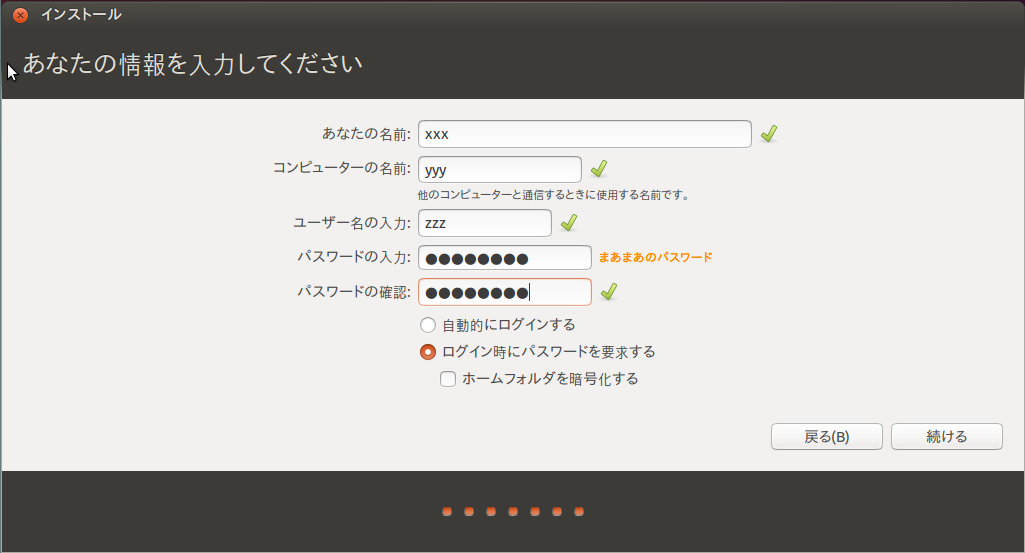
\includegraphics[width=15cm]{ubuntuinstall05.png}
\caption{情報入力画面}\label{情報入力画面}
\end{figure}


数分待機すると,インストールが終了し,以下の画面が表示される.「今すぐ再起動する」をクリックし,画面に表示されるメッセージがとまったら,何か適当かキーを打つ.すると,仮想マシンが再起動する.


\begin{figure}[H]
\centering
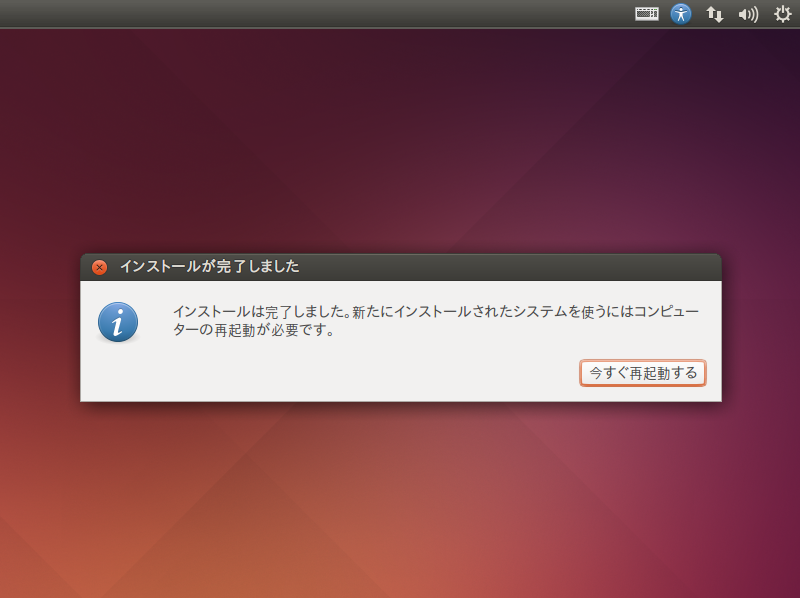
\includegraphics[width=15cm]{ubuntuinstall06.png}
\caption{インストール完了画面}\label{イメージ画面}
\end{figure}

この様な画面が表示されればインストールが終了する.


\begin{figure}[H]
\centering
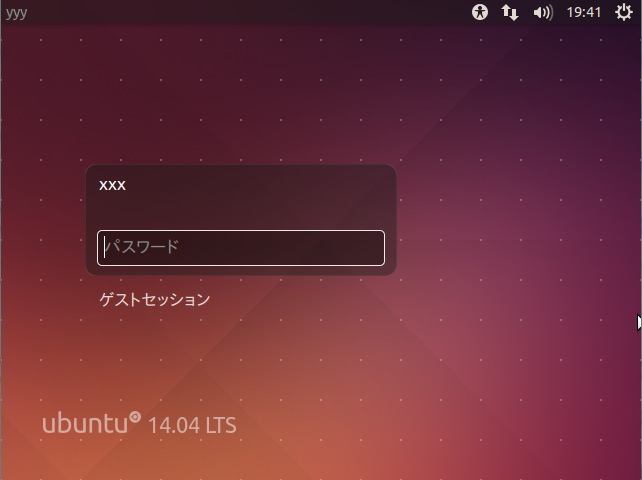
\includegraphics[width=15cm]{ubuntuinstall07.png}
\caption{ログイン画面}\label{イメージ画面}
\end{figure}

\subsubsection{Tweepyのインストール}

Python上でTwitterのAPIを操作し,情報収集をするために,Tweepyというライブラリをインストールする.
まずはデスクトップ上にある端末を選択する.
\begin{figure}[H]
\centering
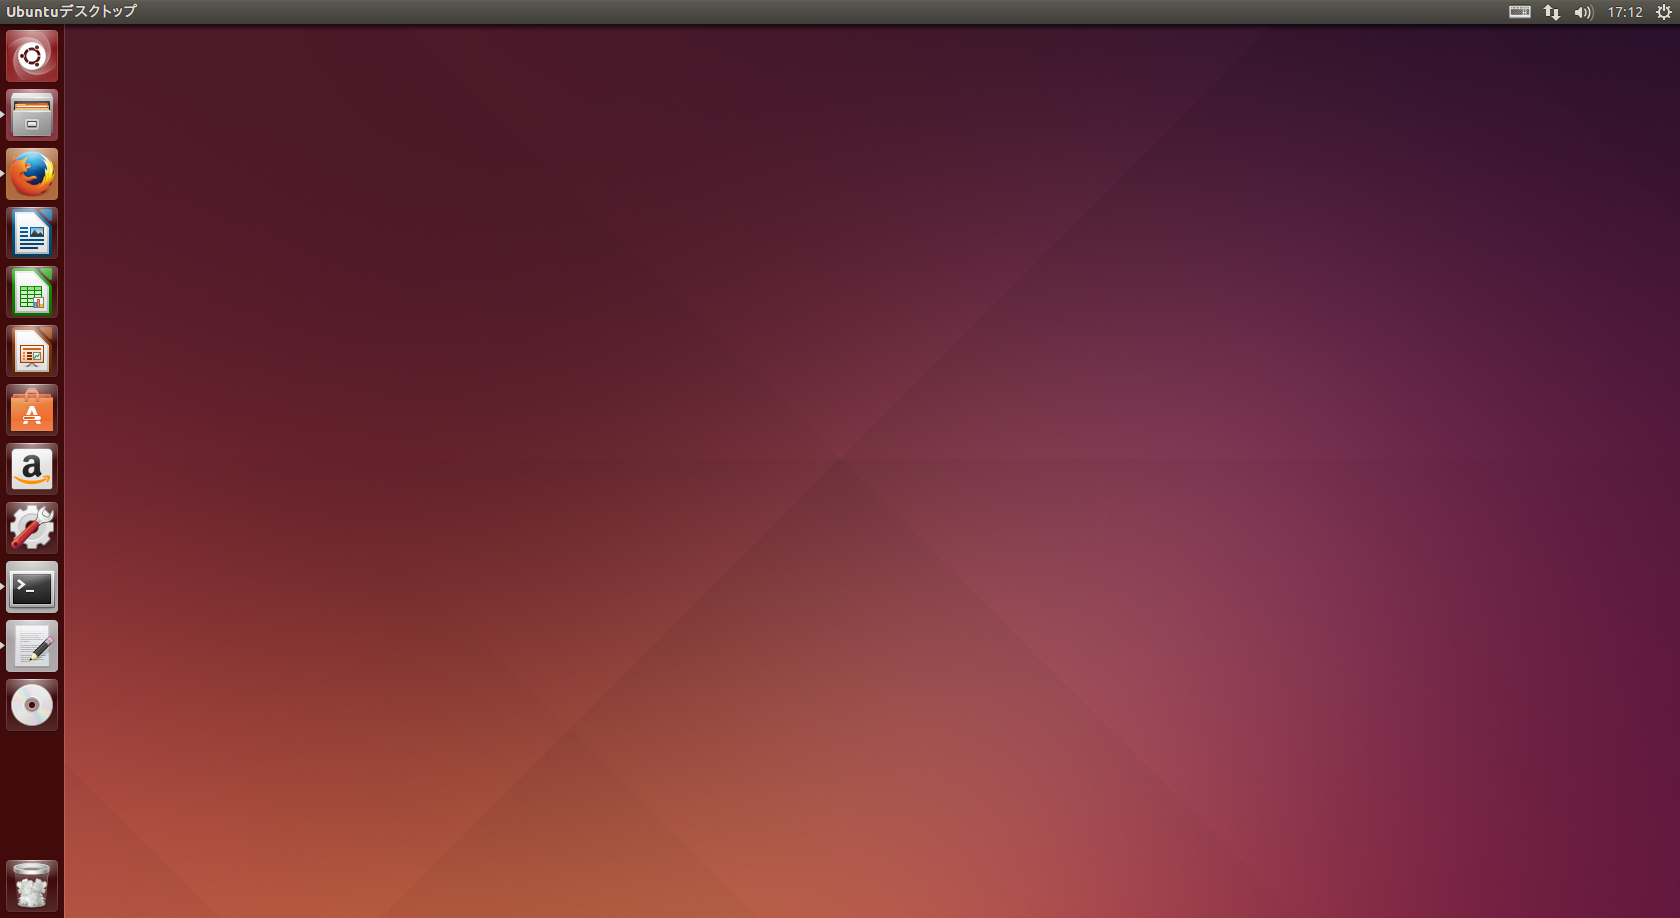
\includegraphics[width=15cm]{tweepyinstall001.png}
\caption{Ubuntu デスクトップ}\label{Ubuntu デスクトップ画像}
\end{figure}

以下の画面が表示される.

\begin{figure}[H]
\centering
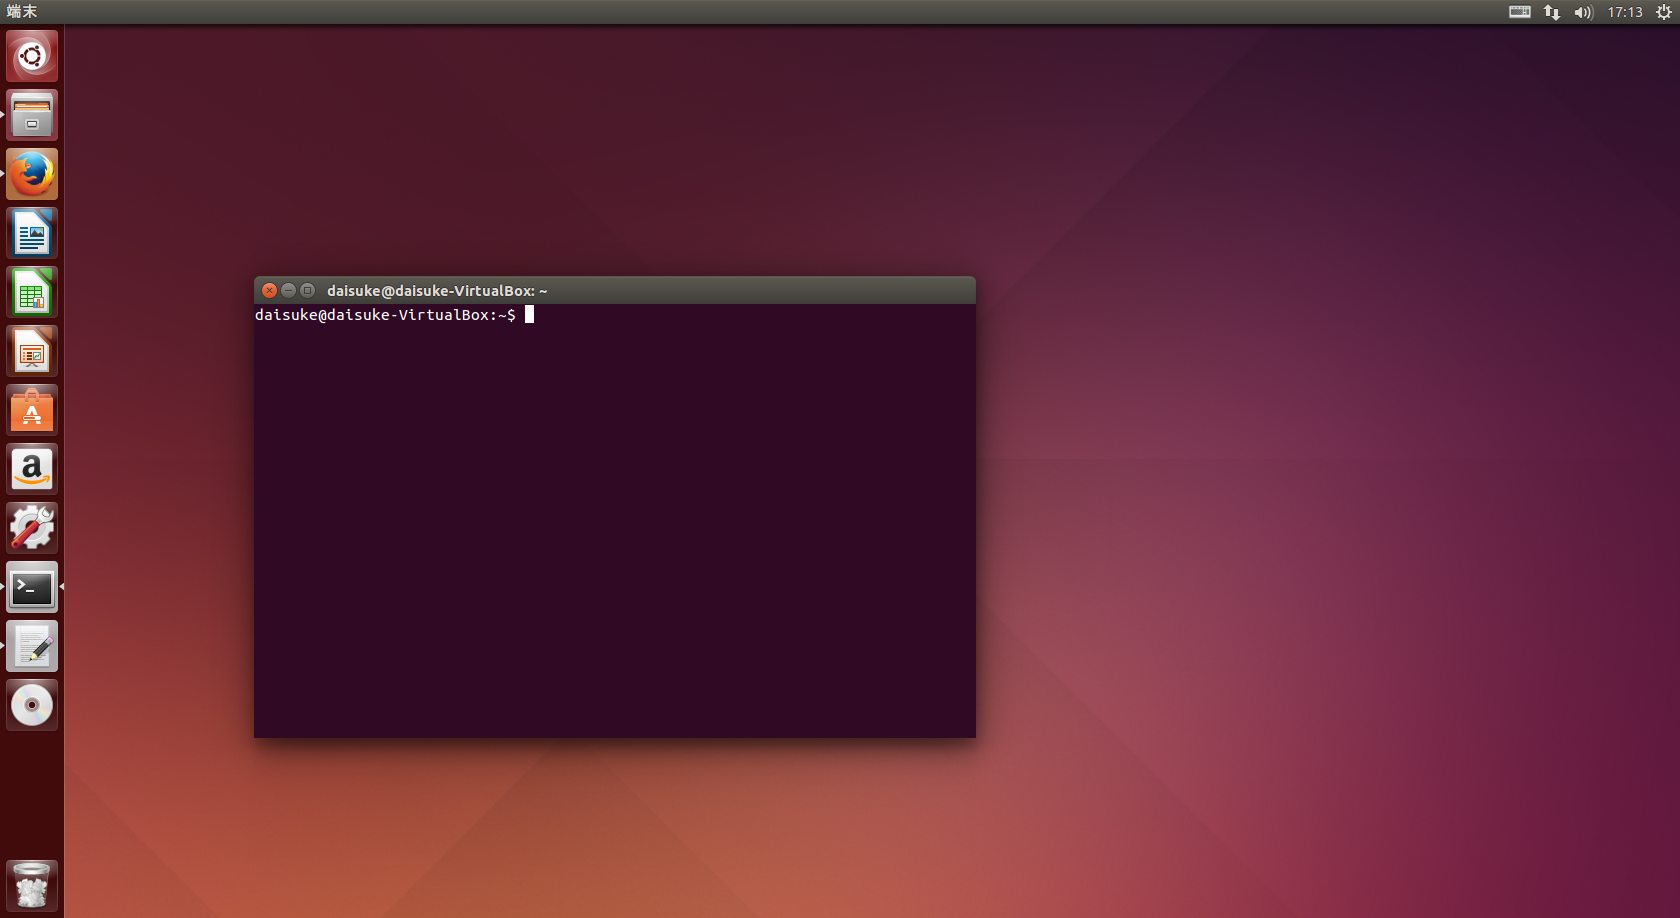
\includegraphics[width=15cm]{tweepyinstall002.png}
\caption{端末画面}\label{Ubuntu端末画面}
\end{figure}

その後端末上で以下のコマンドを入力する.
1行目のコマンドを実行すると,パスワードの入力を求められ,インストールが始まる.その後2行目のコマンドを実行するとインストールが完了する.
\begin{lstlisting}
sudo apt-get install python-setuptools python-pip
sudo easy_install tweepy
\end{lstlisting}


\section{Twitterアカウントと電話番号の紐付け}

開発者向けにTwitterを利用するため,Consumer Key,Consumer Secret,Access Token,Access Token Secretが必要になるため,Twitterアカウントと電話番号を紐付けする必要がある.

\subsection{アプリケーションの利用}
Twitterの開発者向けのページ(https://dev.twitter.com/)にアクセスし,Manage Your Appsをクリックする.

\begin{figure}[H]
\centering
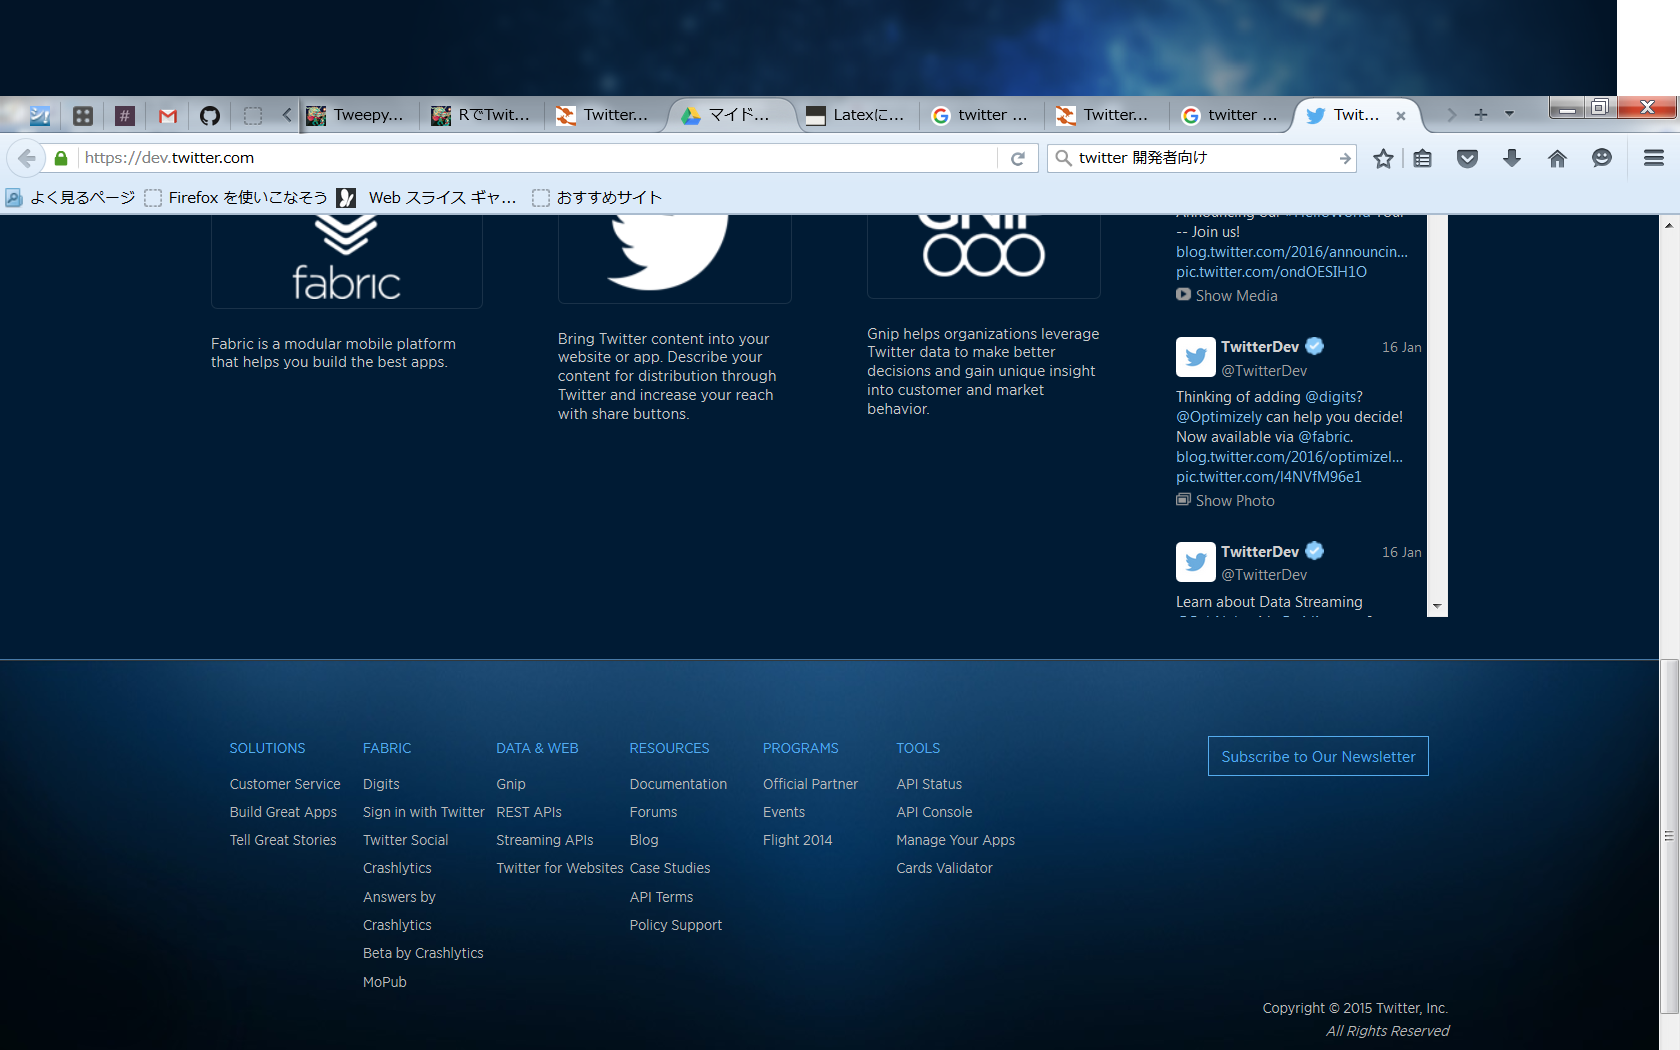
\includegraphics[width=15cm]{twitterdev001.png}
\caption{Twitter開発者向けのページ}\label{Twitter開発者向けページ}
\end{figure}

以下の画面が表示され,右上のCreate New Appをクリックする.

\begin{figure}[H]
\centering
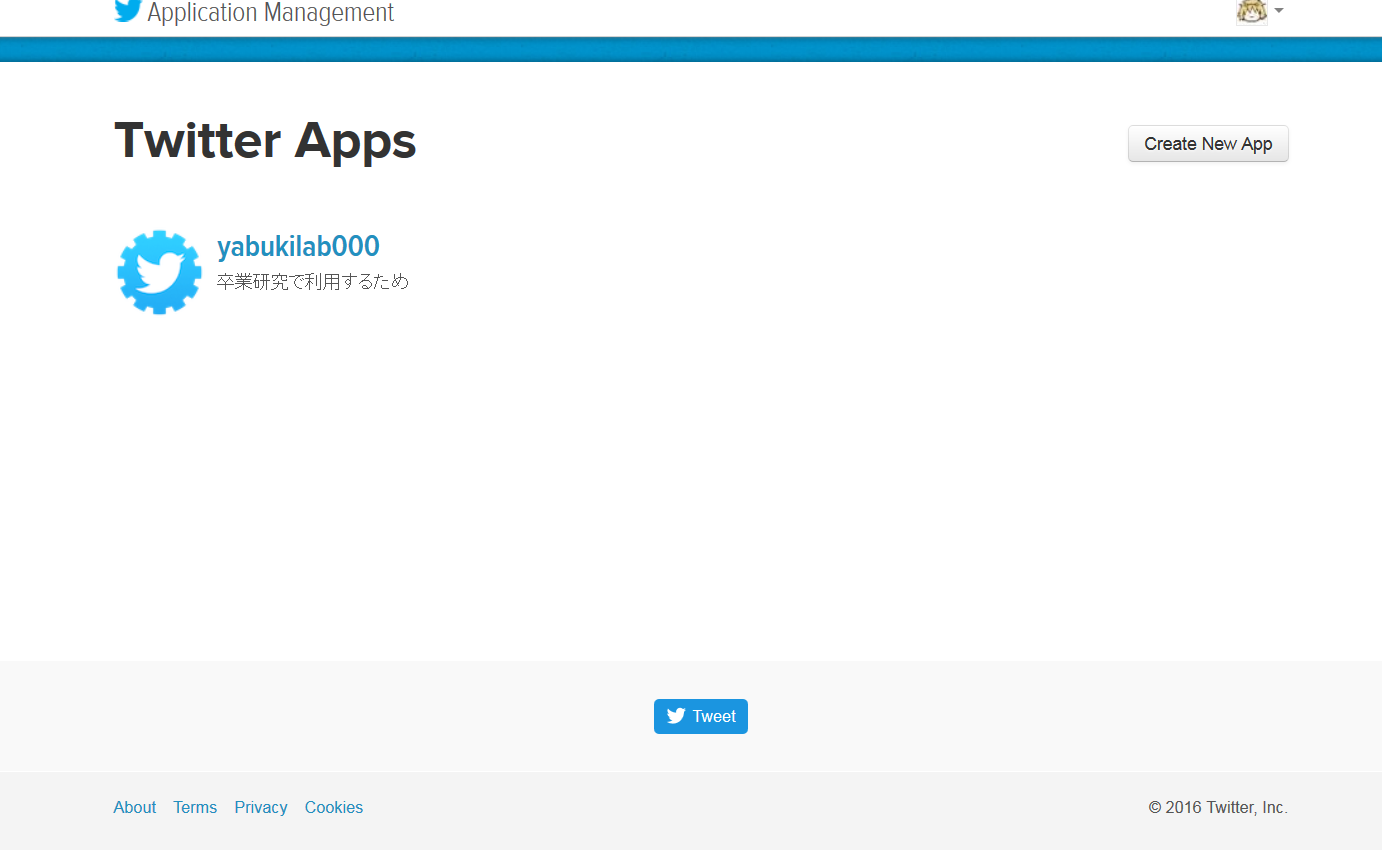
\includegraphics[width=15cm]{twitterdev002.png}
\caption{Twitter開発者向けのページ 2}\label{Twitter開発者向けページ 2}
\end{figure}

この画面に移動し,名前や利用目的などの入力するとアプリケーションが作成され,Consumer Key,Consumer Secret,Access Token,Access Token Secretを取得できる.


\begin{figure}[H]
\centering
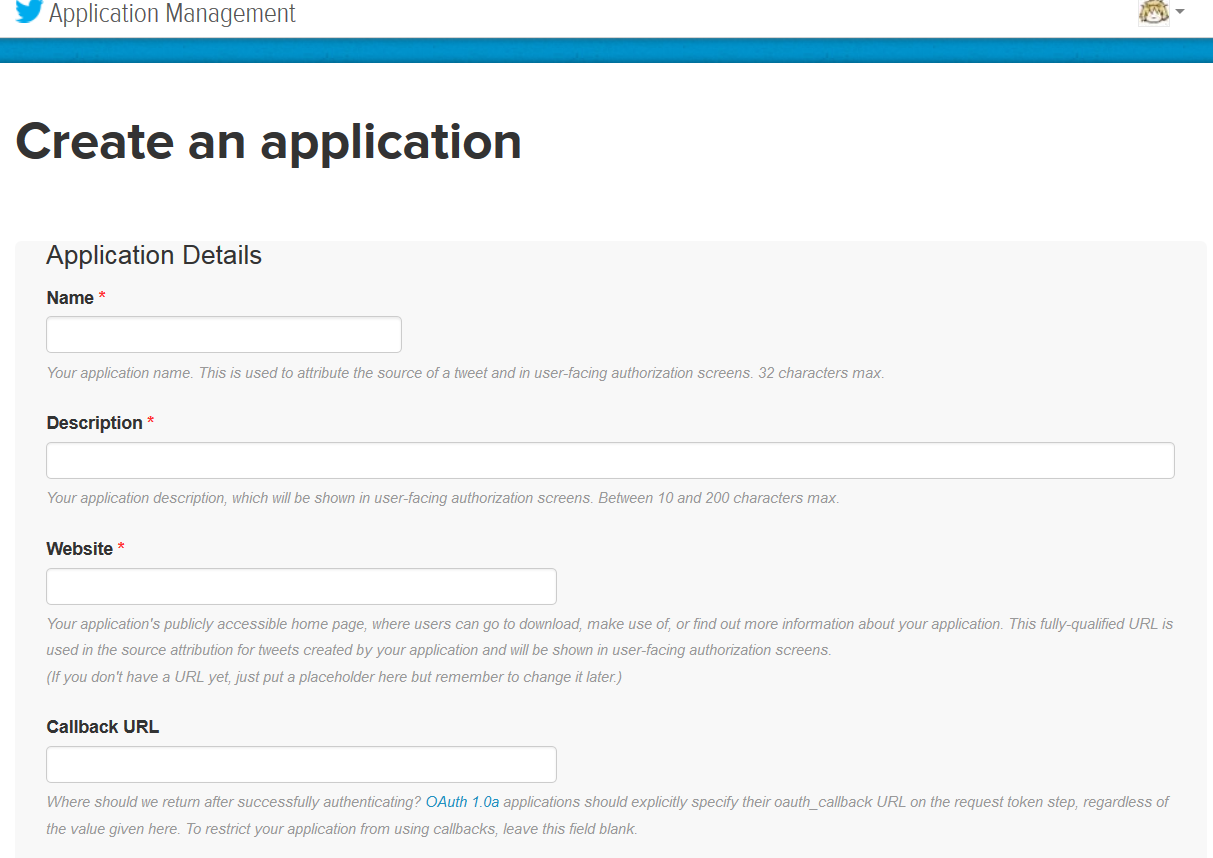
\includegraphics[width=15cm]{twitterdev003.png}
\caption{Twitter開発者向けのページ 3}\label{Twitter開発者向けページ 3}
\end{figure}

\section{端末の使用方法}
本研究ではUbuntu上にある端末を使用する.その端末の使用方法について記述する.

\subsection{端末のコマンド}

\begin{table}[htb]
  \begin{center}
  \begin{tabular}{|l|c|} \hline
    コマンド & 機能 \\ \hline \hline
    ls & ファイルの一覧表示 \\  \hline
    cp & ファイルのコピー \\  \hline
    mv & ファイルの移動,ファイル名の変更 \\ \hline
    rm & ファイルの削除 \\  \hline
    pwd & カレントディレクトリの表示 \\  \hline
    cd & カレントディレクトリの変更 \\ \hline
    cat & ファイルの内容を表示 \\  \hline
   python & pythonプログラムの起動  \\  \hline
   sh & bashプログラムの起動 \\  \hline
  mysql & ユーザー名とパスワードを同時に記載することでmysqlが起動 \\ \hline
  curl & プロトコルを用いてデータを通信するコマンドライン ツール \\  \hline
 echo & 因数に与えられた文字列を表示する \\  \hline
   > & ファイルに出力する \\  \hline
 chmod &ファイルやディレクトリのアクセス権を変更する \\  \hline
 grep & 文字列を検索する \\  \hline
  \end{tabular}
  \end{center}
\end{table}


\clearpage


\chapter{Pythonについて}

\section{本章の構成}
本章では本研究で使用するプログラミング言語,Pythonについて記す.



\section{Pythonとは}
Pythonは,広く使用されている汎用のプログラミング言語であり,コードのリーダビリティが高くなるように言語が設計されていると言われ,その構文のおかげで,C言語に比べて,より少ないコード行数でプログラムを表現できると言われている.小規模なプログラムから大規模なプログラムまで,様々なプロ不ラムをクリアに書けるように,多くのコードが提供されている\cite{Pythonwiki}.


\subsection{Pythonの特徴}

Pythonには次のような特徴がある\cite{Pythontokutyou}.

\begin{itemize}
 \item とてもクリーンで読みやすい文法.
 \item 直感的なオブジェクト指向
 \item 手書き方のコードによる自然な表現
 \item パッケージの階層化もサポートした,完全なモジュール化サポート
 \item Windows,Linux/Unix,OS/2,Mac,Amigaなどの多くのメジャーなOSで使うことができる,1度書いたソースコードが,変更なしで動く.
 \item Pythonの実装は自由に使用でき,自由に配布でき,商用利用も可能なオープンなソースライセンスで提供されている.
\end{itemize}

\clearpage


\section{ツイートの取得}

Ubuntuの端末を起動して,以下のプログラム(stream.py)を実行する.Consumer KeyとConsumer Secret,Acces Token,Access Token Secretは先ほど取得したものを入力する.「python stream.py >>result.dat」を入力し実行するとそのつぶやきresult.datに書き込まれる.
{\small
\begin{lstlisting}
 -*- coding: utf-8 -*-
 
from tweepy.streaming import StreamListener
from tweepy import OAuthHandler
from tweepy import Stream
 
consumer_key = ""
consumer_secret = ""
 
access_token = ""
access_token_secret = ""
 
class StdOutListener(StreamListener):
    def on_data(self, data):
        if data.startswith("{"):
            print data
        return True
 
    def on_error(self, status):
        print status
 
if __name__ == '__main__':
    l = StdOutListener()
    auth = OAuthHandler(consumer_key, consumer_secret)
    auth.set_access_token(access_token, access_token_secret)
 
    stream = Stream(auth, l)
    stream.sample(track = [keyword])
\end{lstlisting}}

\begin{figure}[H]
\centering
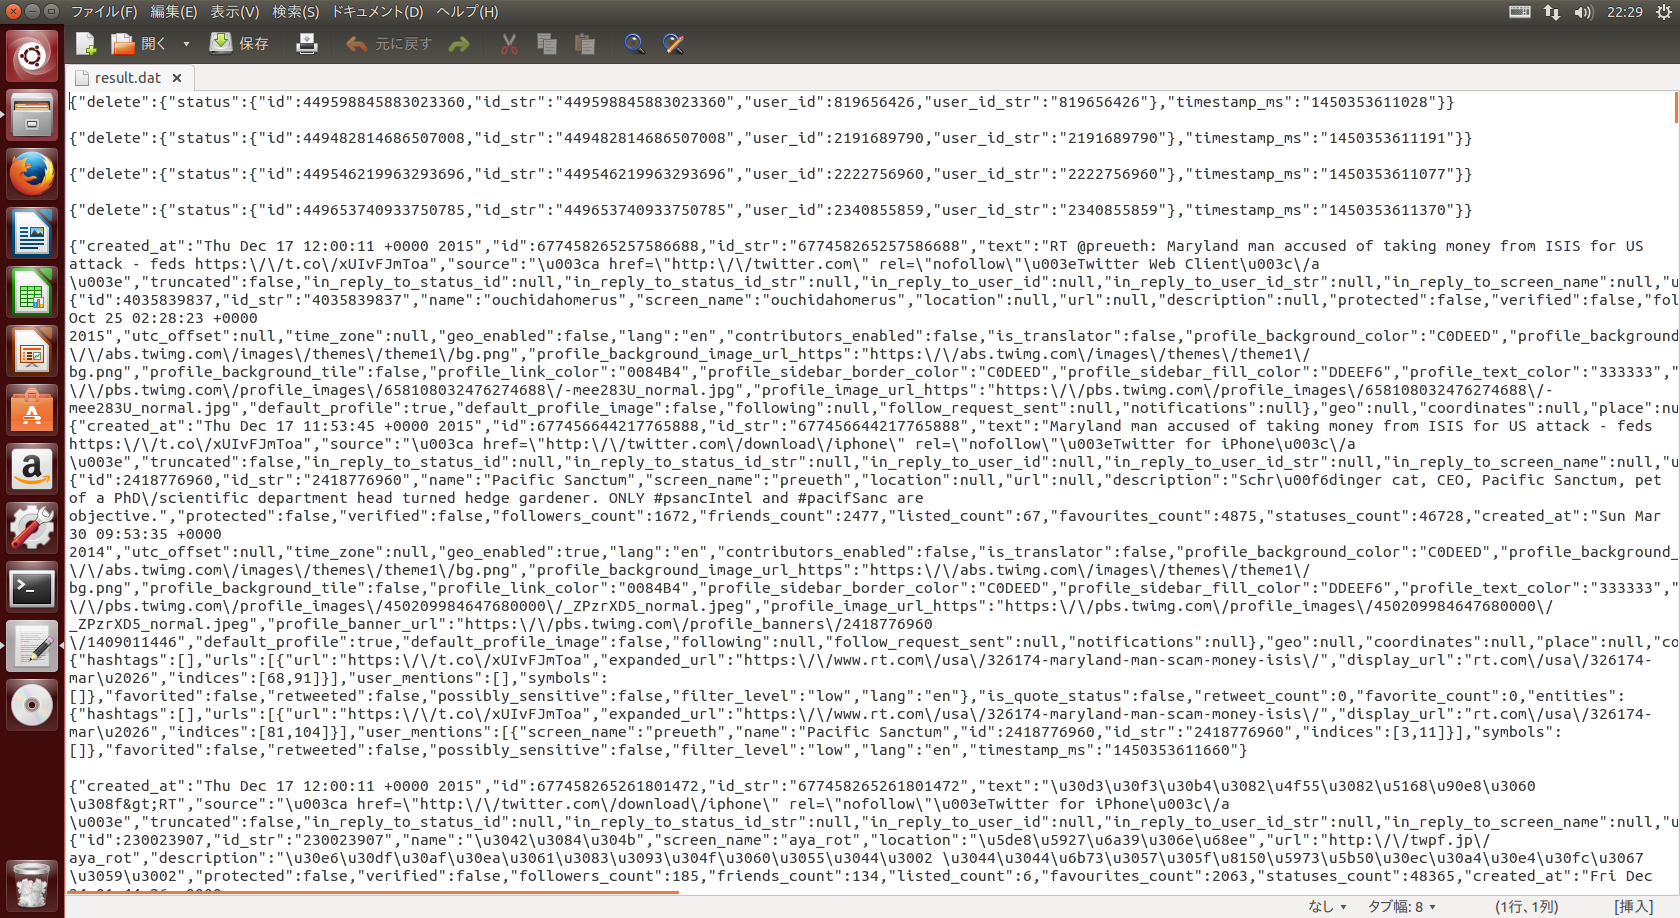
\includegraphics[width=15cm]{resultdat.png}
\caption{result.dat}\label{result.datの画像}
\end{figure}


\clearpage


\section{ツイートの処理}

以下のプログラムを実行する(parse.py)を使えば時間指定などを指定し,その時間内のつぶやきだけを取得することができる.
日本時間の2015年12月1日12時00分から,2015年12月2日12時00分までのつぶやきを取得したいのならば,「python parse.py 20151201120000 20151202120000 < result.dat」を端末に入力し実行すればよい.


{\small
\begin{lstlisting}
#!/usr/bin/env python
import sys, json, time, calendar
#from pprint import pprint
 
def YmdHMS(created_at):
    time_utc = time.strptime(created_at, '%a %b %d %H:%M:%S +0000 %Y')
    unix_time = calendar.timegm(time_utc)
    time_local = time.localtime(unix_time)
    return int(time.strftime("%Y%m%d%H%M%S", time_local))
 
argv = sys.argv
start_time = 0
end_time = 99999999999999
if 1 < len(argv):
    start_time = int(argv[1])
    end_time = int(argv[2])
 
for line in sys.stdin:
    try:
        tweet = json.loads(line)
        #pprint(tweet)
        if 'retweeted_status' not in tweet:
            tweet_time = YmdHMS(tweet['created_at'])
            if start_time <= tweet_time and tweet_time <= end_time:
                tweet_sec = tweet_time-start_time
                screen_name = tweet['user']['screen_name']
                text = tweet['text'].encode('utf-8')
                url = "https://twitter.com/#!/%s/status/%s"\
                    % (screen_name, tweet['id_str'])
                #print tweet_sec, url, text
                #print text
                t = time.strptime(str(tweet_time), "%Y%m%d%H%M%S")
                print time.strftime("%H:%M:%S", t), text
    except StandardError:
        pass
\end{lstlisting}}

\clearpage

\section{OAuth認証}
OAuthとは,Webサーバーにあるユーザーのリソースへのアクセス権限を,ユーザーの代理で行うことを許可するための認証用のプロトコルのことである.
OAuthを使用することで,エンドユーザーはクライアントにユーザ名やパスワードを知らせることなく,サーバーリソースへの第三者アクセスを認可することができる.OAuthでは,ログインのために必要なユーザー名とパスワードをユーザー毎に割り当てるトークンと呼ばれる情報に置き換えて使う.このトークンを使うことで外部のサービスにはパスワードを教えることなく,システム間の情報の共有が可能になる\cite{OAuth}.
以下のプログラムからOAuthのための情報を入力する.

\begin{lstlisting}
# -*- coding: utf-8 -*-

import tweepy

consumer_key = ""
consumer_secret = ""

access_token = ""
access_token_secret = ""

auth = tweepy.OAuthHandler(consumer_key, consumer_secret)
auth.set_access_token(access_token, access_token_secret)
api = tweepy.API(auth)
\end{lstlisting}

\section{データベースの作成}

今回はTwitterのツイートを集めて管理する.収集したデータを簡単に検索、抽出できるようにデータベースを作成する.そのために以下のプログラムをUbuntuの端末から実行する.





\begin{lstlisting}
 sudo apt-get install mysql-server mysql-client


 mysql -uroot -ppass

drop database if exists twitter;
create database twitter default charset=utf8;


grant all on twitter.* to test@localhost identified by 'pass';

use twitter;


drop table if exists users;
create table users (
  id bigint primary key,
  screenName varchar(100) not null,
  statuses int,
  friends int,
  followers int,
  lang varchar(10),
  profileImageUrl varchar(1000),
  rekognition text,
  index(lang),
  unique index(screenName)
);

desc users;


drop table if exists retweets;
create table retweets (
  id bigint primary key,
  retweet bigint not null,
  retweeted bigint not null,
  rcount int not null,
  fcount int not null,
  foreign key (retweet) references users (id),
  foreign key (retweeted) references users (id),
  unique index(retweet,retweeted)
);

desc retweets;


drop table if exists retweeters;
create table retweeters (
  id int auto_increment primary key,
  tweetId bigint not null,
  retweet bigint not null,
  foreign key (tweetId) references retweets (id),
  foreign key (retweet) references users (id)
);

desc retweeters;


drop table if exists friends;
create table friends (
  id int auto_increment primary key,
  user bigint not null,
  friend bigint not null,
  foreign key (user) references users (id),
  index(friend)
);

desc friends;


alter table users add friendsChecked boolean not null default false;
alter table users add index(friendsChecked);
alter table retweets add retweetersChecked boolean not null default false;
alter table retweets add index(retweetersChecked);


update users set friendsChecked = true where exists (select * from friends where friends.user=users.id);


update retweets set retweetersChecked = true where exists (select * from retweeters where retweeters.tweetId = retweets.id);


\end{lstlisting}

1行目のsudo apt-get install mysql-server mysql-clientを入力すると,パスワードの入力を求められ,入力するとデータベースをインストールされる.

\begin{figure}[H]
\centering
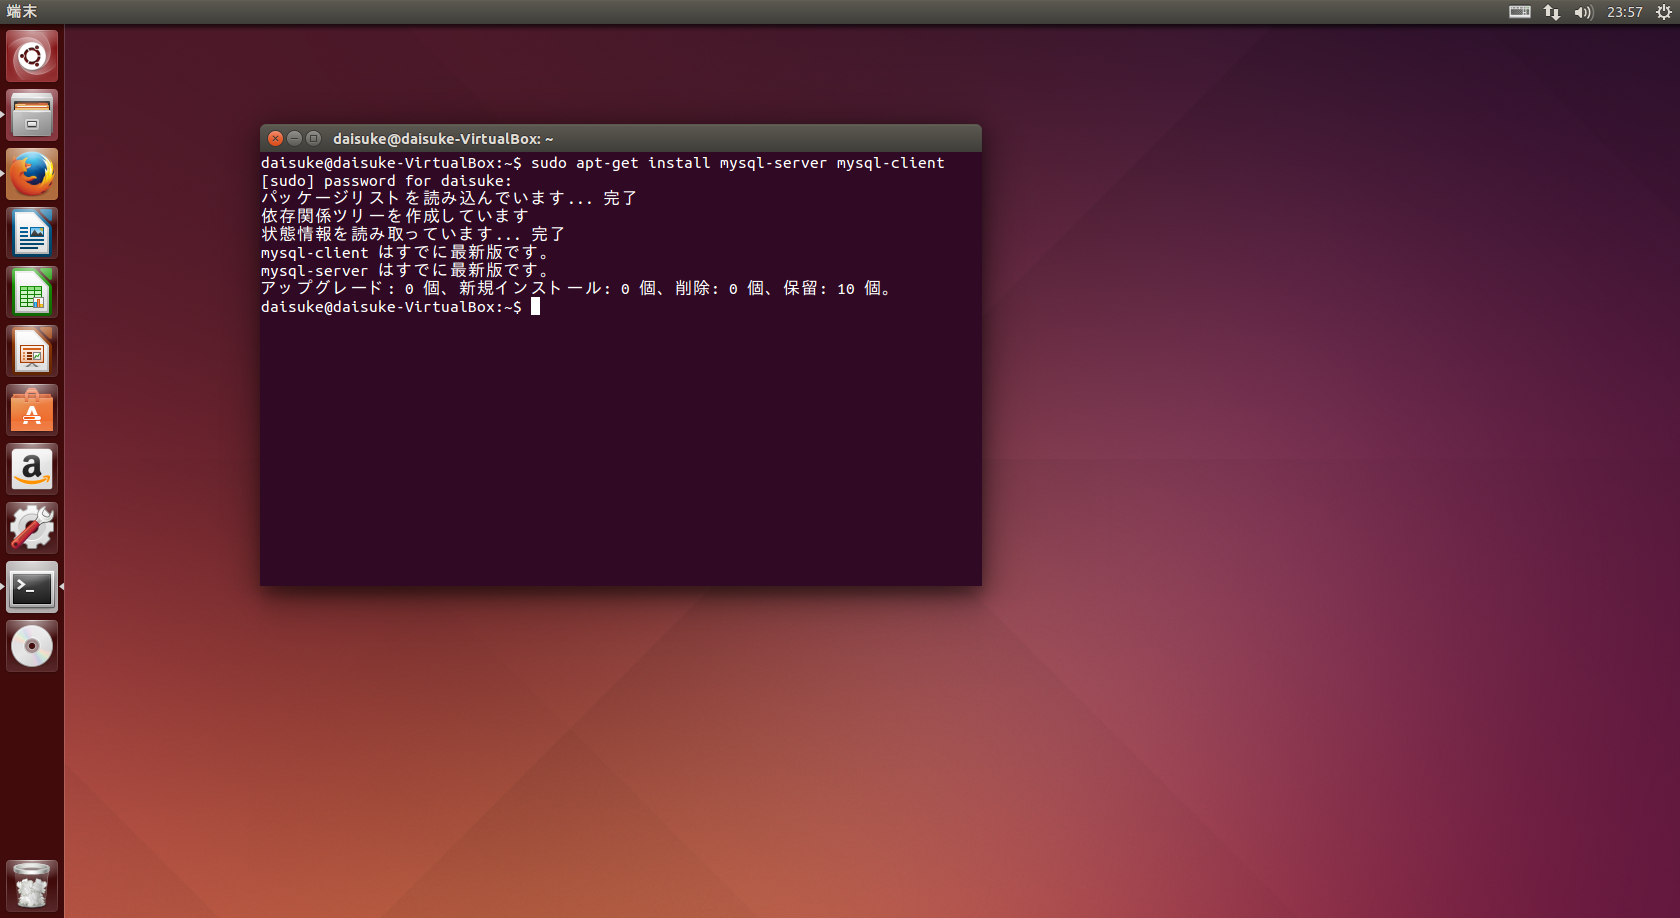
\includegraphics[width=15cm]{database001.png}
\caption{データベース1}\label{データベース001の画像}
\end{figure}

その後のmysql -uroot -ppassで管理者のrootのパスワードを決める.今回はpassとする.

\begin{figure}[H]
\centering
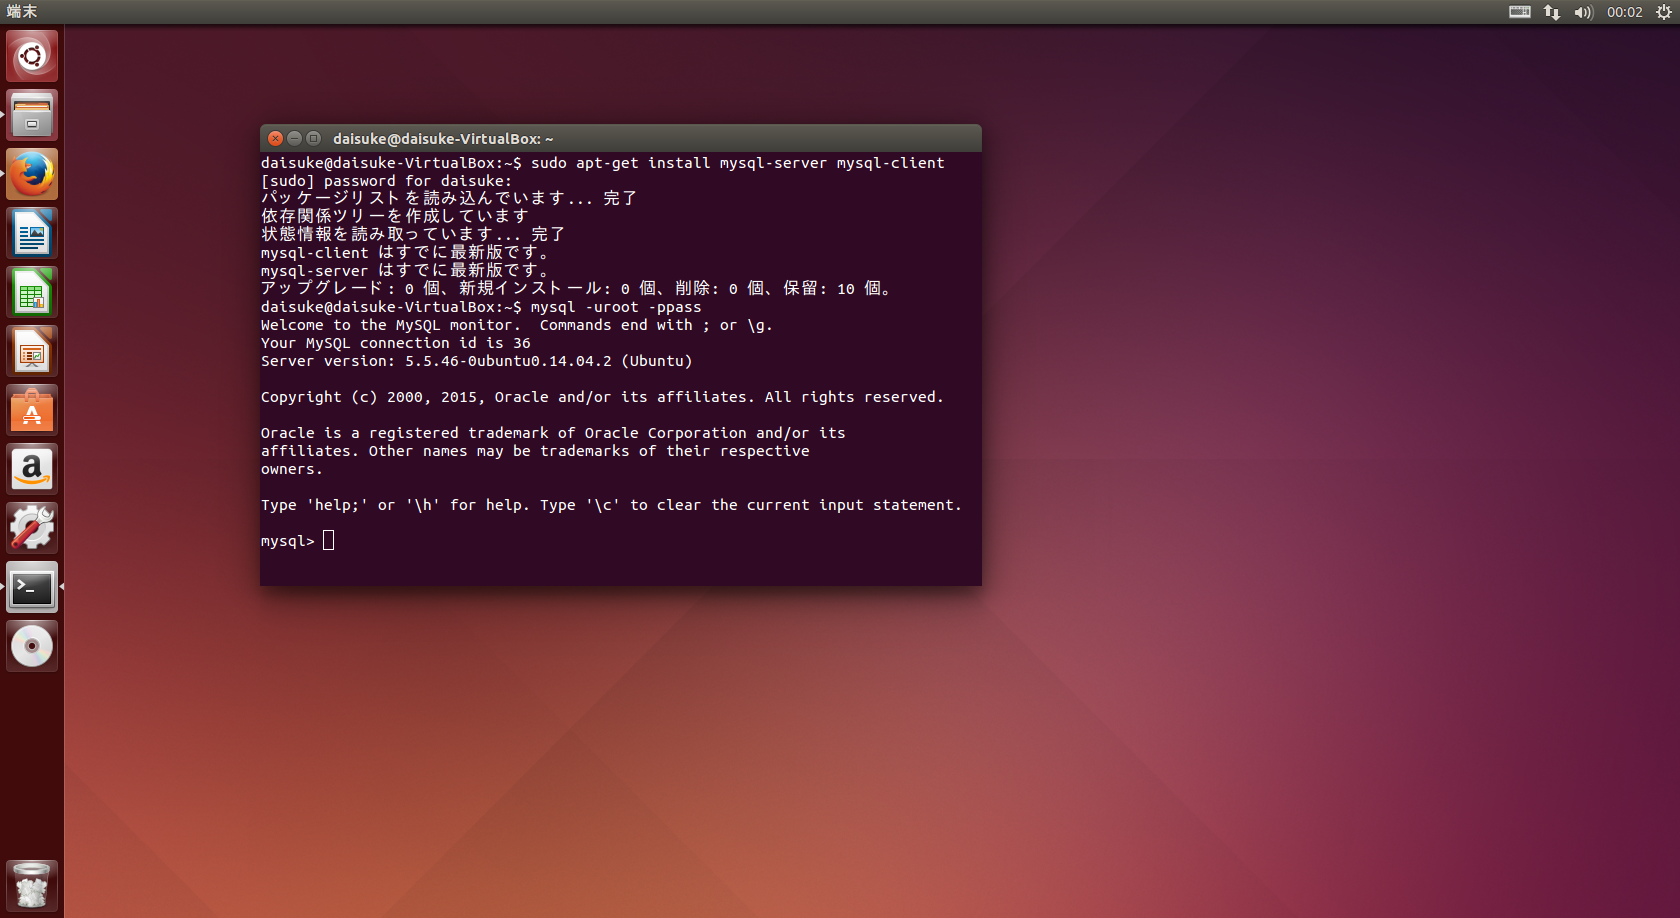
\includegraphics[width=15cm]{database002.png}
\caption{データベース2}\label{データベース002の画像}
\end{figure}

desc users;を端末に入力することでユーザを記録したテーブルを参照でき,desc retweets;でリツイートを記録したテーブルを参照できる.

\begin{figure}[H]
\centering
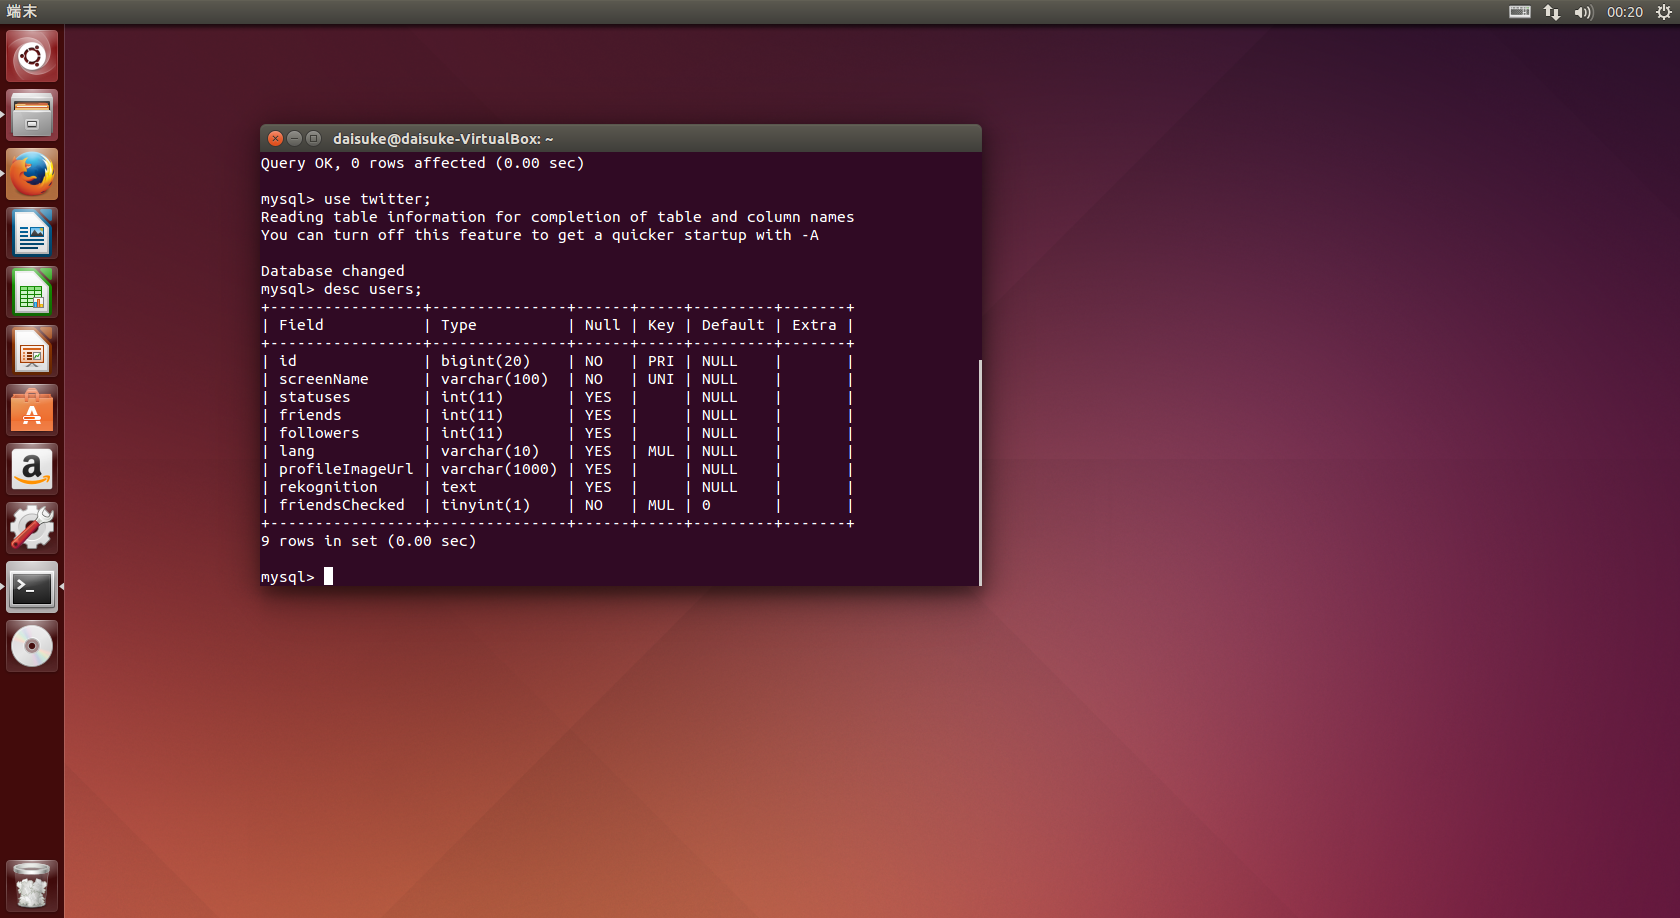
\includegraphics[width=15cm]{database003.png}
\caption{ユーザテーブル}\label{データベース003の画像}
\end{figure}


\begin{figure}[H]
\centering
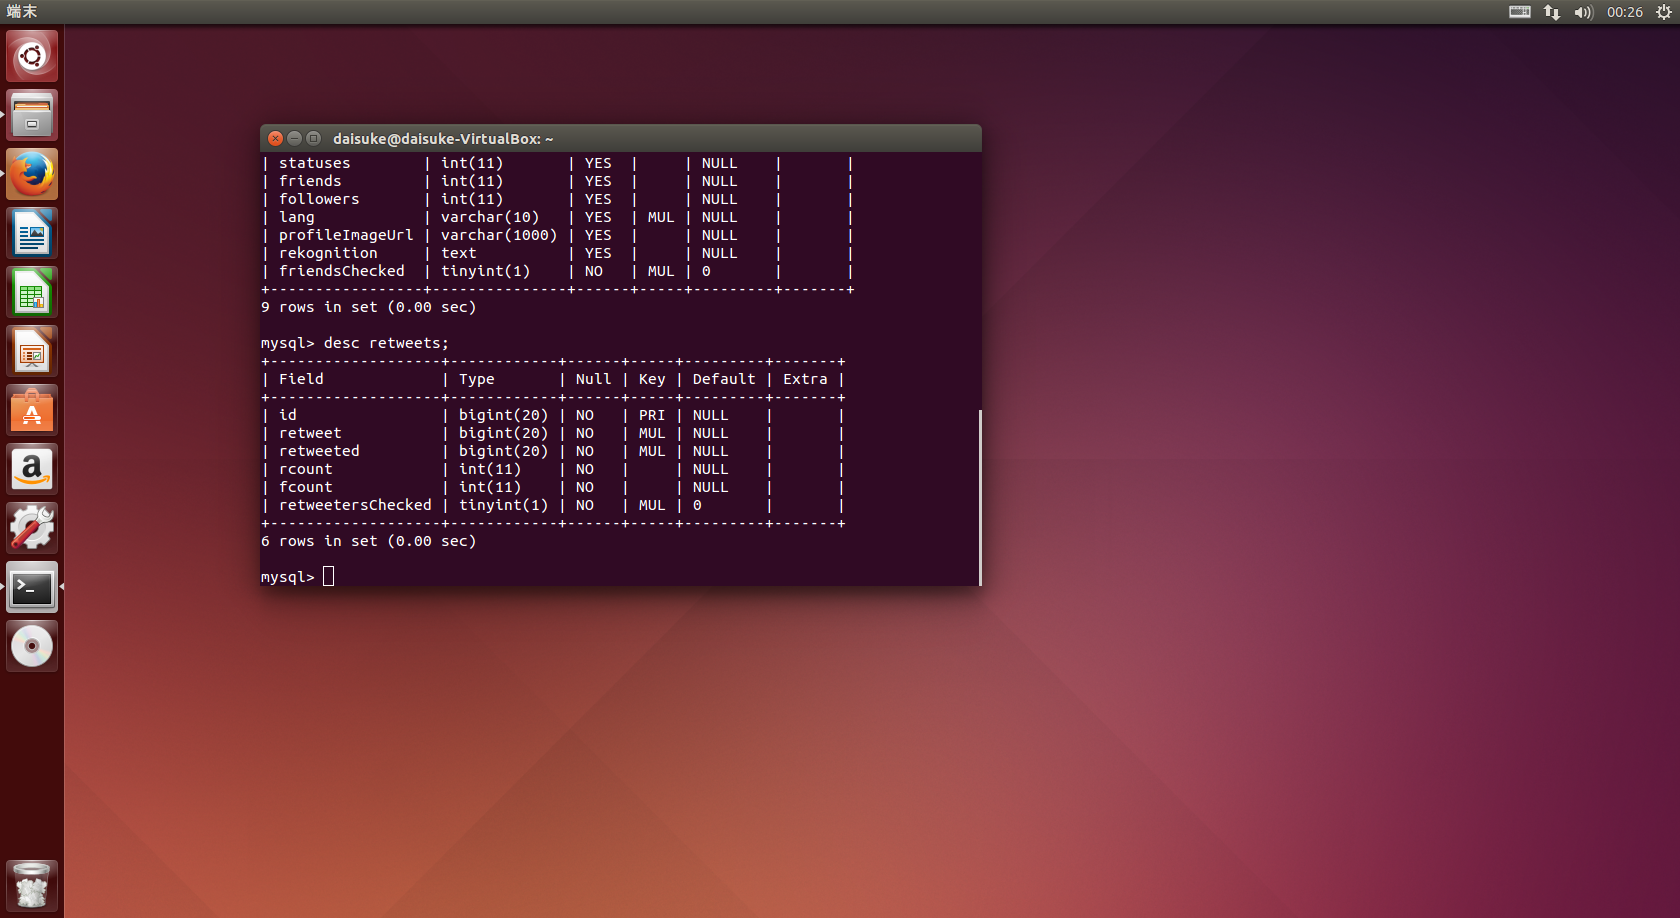
\includegraphics[width=15cm]{database004.png}
\caption{リツイートテーブル}\label{データベース004の画像}
\end{figure}


grant all on twitter.* to test@localhost identified by 'pass';でユーザをtest,パスワードをpassでアクセスできるようにする.

\clearpage

\section{リツイートの記録}

\subsection{本章の構成}
本章ではリツイートを記録する方法を記述する.

\subsection{手順1}
streamingしたデータを標準出力に書き出す必要があり,そのために以下のプログラム(stream.py)をつくる.
その後,Ubuntuの端末に(python stream.py)を入力すると書き出される.
\begin{lstlisting}

 -*- coding: utf-8 -*-
 
from tweepy.streaming import StreamListener
from tweepy import OAuthHandler
from tweepy import Stream
from auth import auth
 
class StdOutListener(StreamListener):
    def on_data(self, data):
        if data.startswith("{"):
            print data
        return True
 
    def on_error(self, status):
        print status
 
if __name__ == '__main__':
    stream = Stream(auth, StdOutListener())
   stream.sample()

\end{lstlisting}

\begin{figure}[H]
\centering
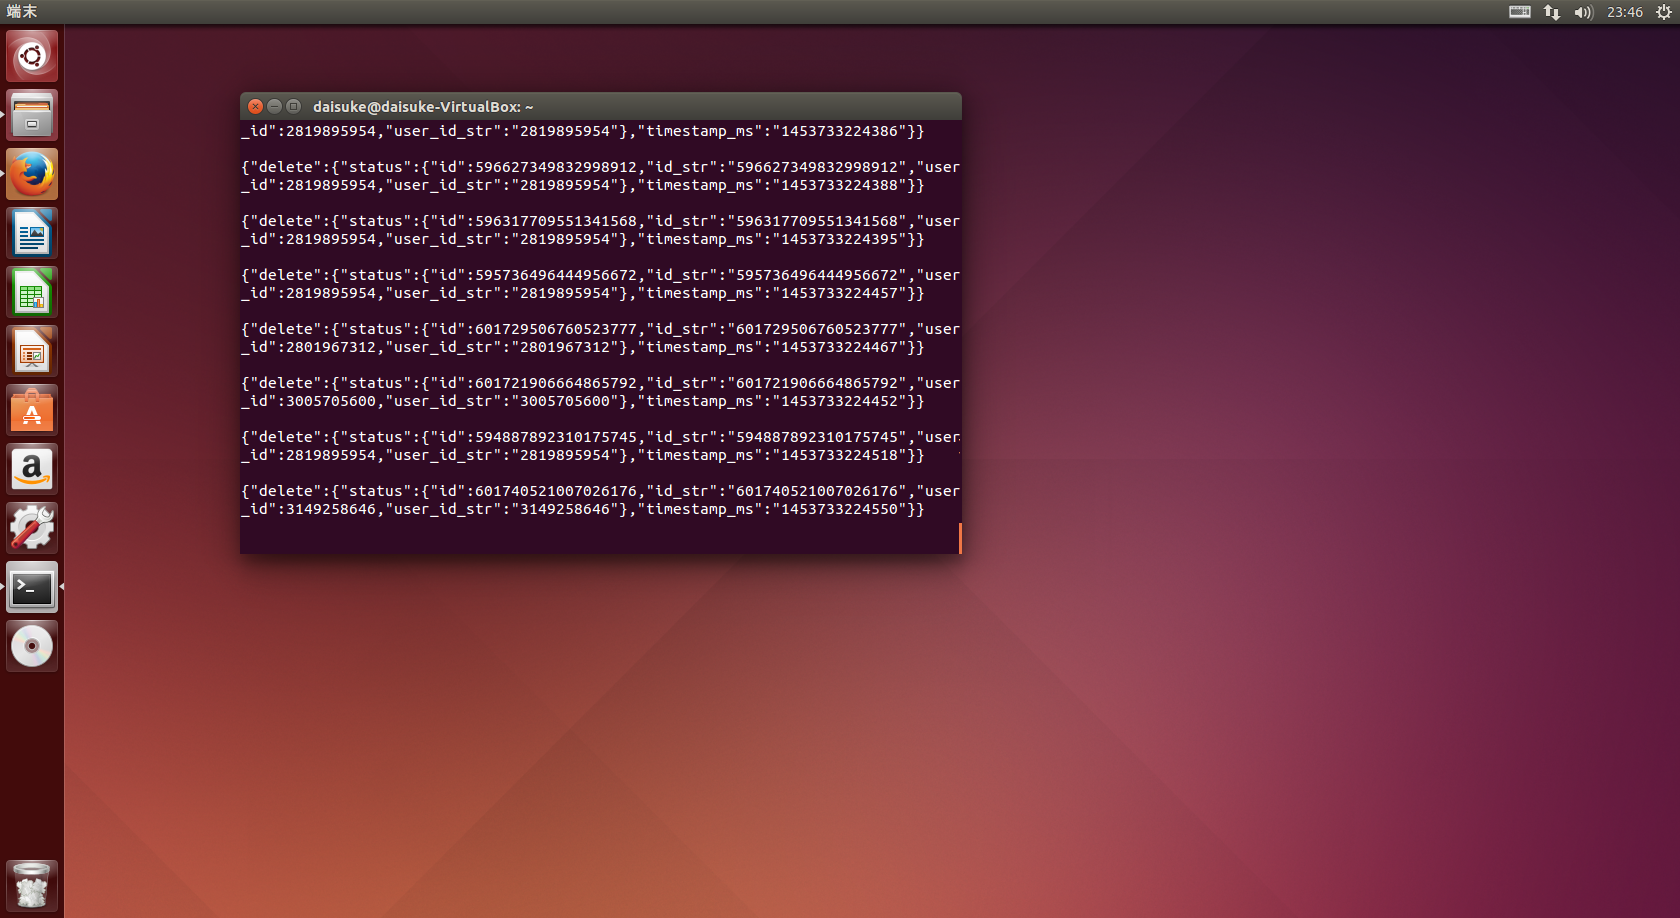
\includegraphics[width=15cm]{streampy.png}
\caption{端末上での動作}\label{stream.pyの画像}
\end{figure}



\subsection{手順2}
手順1で標準出力したデータから,リツイートを抜き出し,データベースに記録するために以下のプログラム(retweets.py)を作る.その後Ubuntuの端末上で(python stream.py | python retweets.py)と入力すれば,リツイートを抜き出し,データベースに記録される.

\begin{lstlisting}

 -*- coding: utf-8 -*-
!/usr/bin/env python
import sys, json
from pprint import pprint

def extractUserProfile(user):
  id = user['id_str']
  screenName = user['screen_name']
  statuses = user['statuses_count']
  friends = user['friends_count']
  followers = user['followers_count']
  lang = user['lang']
  profileImage = user['profile_image_url'].replace('_normal.', '.')
  sys.stdout.write("insert into users (id,screenName,statuses,friends,followers,lang,profileImageUrl) values (%s,'%s',%d,%d,%d,'%s','%s');\n" % (id, screenName, statuses, friends, followers, lang, profileImage))
  return id

for line in sys.stdin:
  try:
    tweet = json.loads(line)
    #pprint(tweet)
    if 'retweeted_status' in tweet:
      #pprint(tweet)
      
      retweet = extractUserProfile(tweet['user'])
      
      retweetedStatus = tweet['retweeted_status']
      tweet = retweetedStatus['id_str']
      rcount = retweetedStatus['retweet_count']
      fcount = retweetedStatus['favorite_count']
      retweeted = extractUserProfile(retweetedStatus['user'])

      sys.stdout.write("insert into retweets (id,retweet,retweeted,rcount,fcount) values (%s,%s,%s,%d,%d);\n" % (tweet, retweet, retweeted, rcount, fcount))
      sys.stdout.flush()
  except ValueError:
    pass

\end{lstlisting}

\begin{figure}[H]
\centering
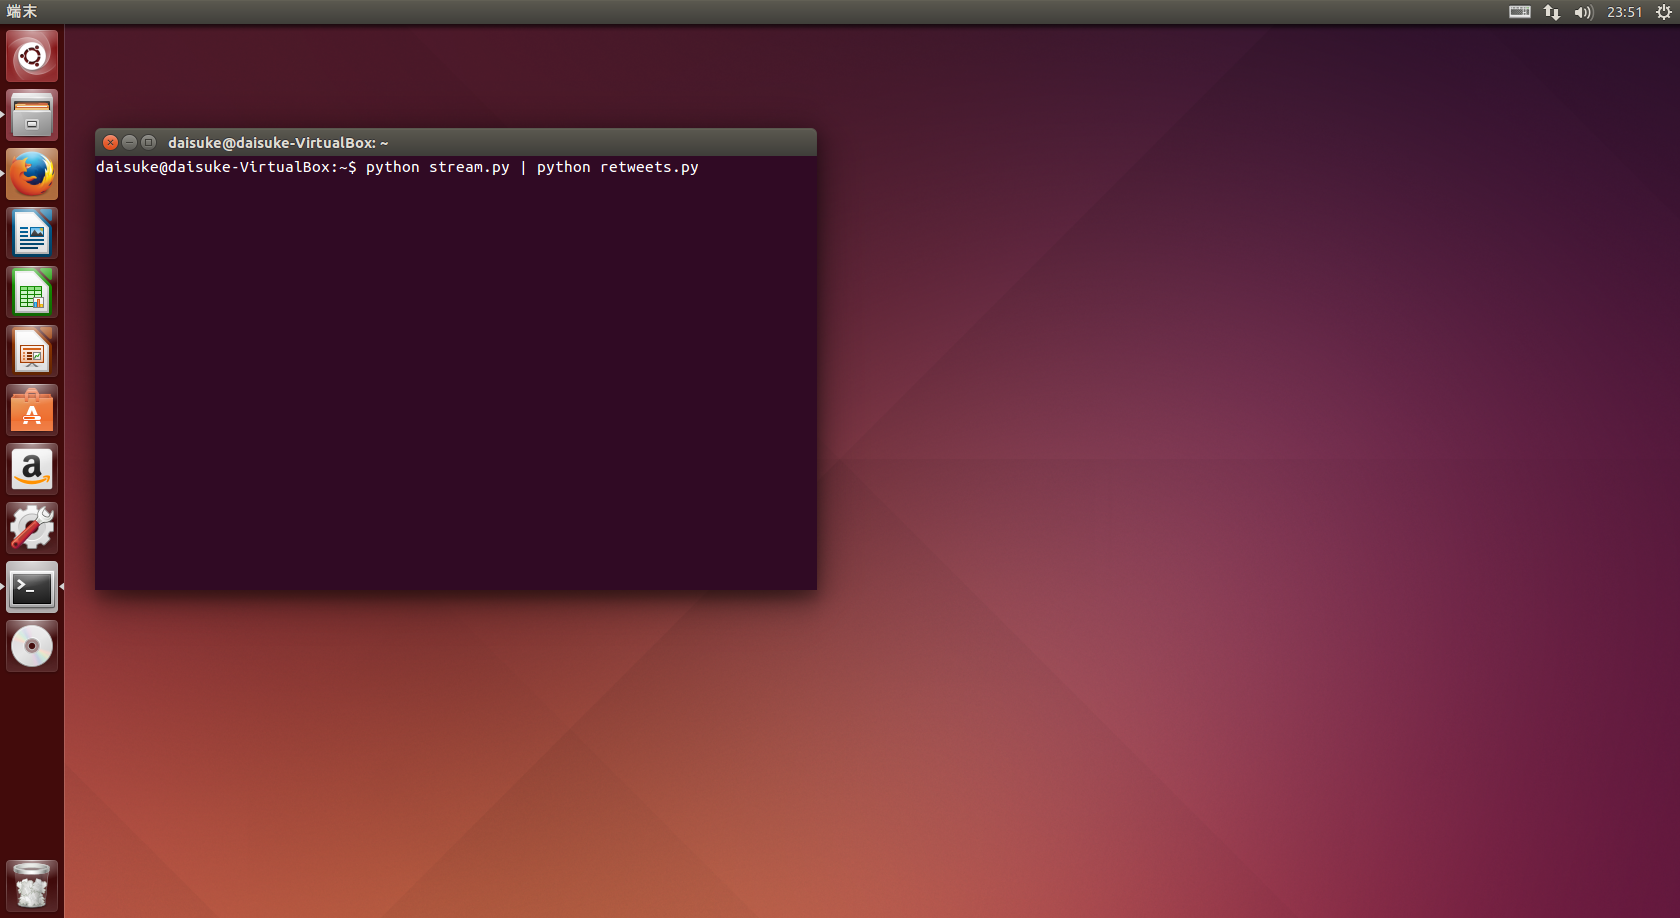
\includegraphics[width=15cm]{retweetspy.png}
\caption{入力画面}\label{retweets.pyの画像}
\end{figure}




\subsection{手順3}
データベースに記録する.

端末上で(python stream.py | python retweets.py | mysql -utest -ppass --force twitter)と入力し,データベースに記録する.
--forceをつけることにより,集めたデータに重複が出た場合のエラーが出ても止まらないようにするためである.

\clearpage

\section{リツイートに関する調査}

\subsection{本章の構成}
本章ではリツイートに関する調査について記述する.

\subsection{リツイートした人がフォローしている人数の取得}
指定したIDのユーザがフォローしている人数を取得するために以下のプログラム(friends.py)を作成する.

\begin{lstlisting}
 -*- coding: utf-8 -*-

import tweepy
import json
import sys
from pprint import pprint
from auth import api

for line in sys.stdin:
  userId = line.rstrip()
  sys.stderr.write("checking friends of %s...\n" % userId)
  
  
  sys.stdout.write("update users set friendChecked=true where id=%s;\n" % (userId))
  
  try:
    friends = api.friends_ids(userId)
    for friendId in friends:
      sys.stdout.write("insert into friends (user,friend) values (%s,%s);\n" % (userId, friendId))
    sys.stdout.flush()
  except:
    pass

\end{lstlisting}

Ubuntuの端末に(echo XXXXX | python friends.py | mysql -utest -ppass --force twitter)と入力する(XXXXXはユーザID)と,指定したIDのユーザがフォローしている人を取得する.また,usersに実在するIDを使わなければ外部キーエラーになるのでデータベースに登録したデータを使う.

データベースから未調査のリツイートを取得するために(echo "select retweet from retweets join users on users.id=retweets.retweet where users.friendsChecked=false limit 1;" | mysql -utest -ppass --skip-column-names twitter | python friends.py | mysql -utest -ppass --force twitter)をUbuntuの端末に入力する.


\chapter{R言語について}
\section{本章の構成}
本章ではR言語について記述する.

\section{R言語とは}
R言語は,ニュージーランドのオークランド大学のRoss IhakaとRobert Clifford Gentlemanにより作られた.\cite{Rgengo}

データ分析やデータ処理に特化したオープンソースのプログラミング言語であり,システム開発をするほかのプラグらミング言語とは位置づけが異なり,統計解析機能が付いていて,分析処理や,その結果をグラフィカルに表示することができる\cite{Rsetumei}.

\section{Rの導入}

R言語はWindows,Macなどの様々なOSで使用可能である.今回では,Windows版での導入方法を記述する.まずR project(https://www.r-project.org/)にアクセスし,右上のCRANをクリックする.



\begin{figure}[H]
\centering
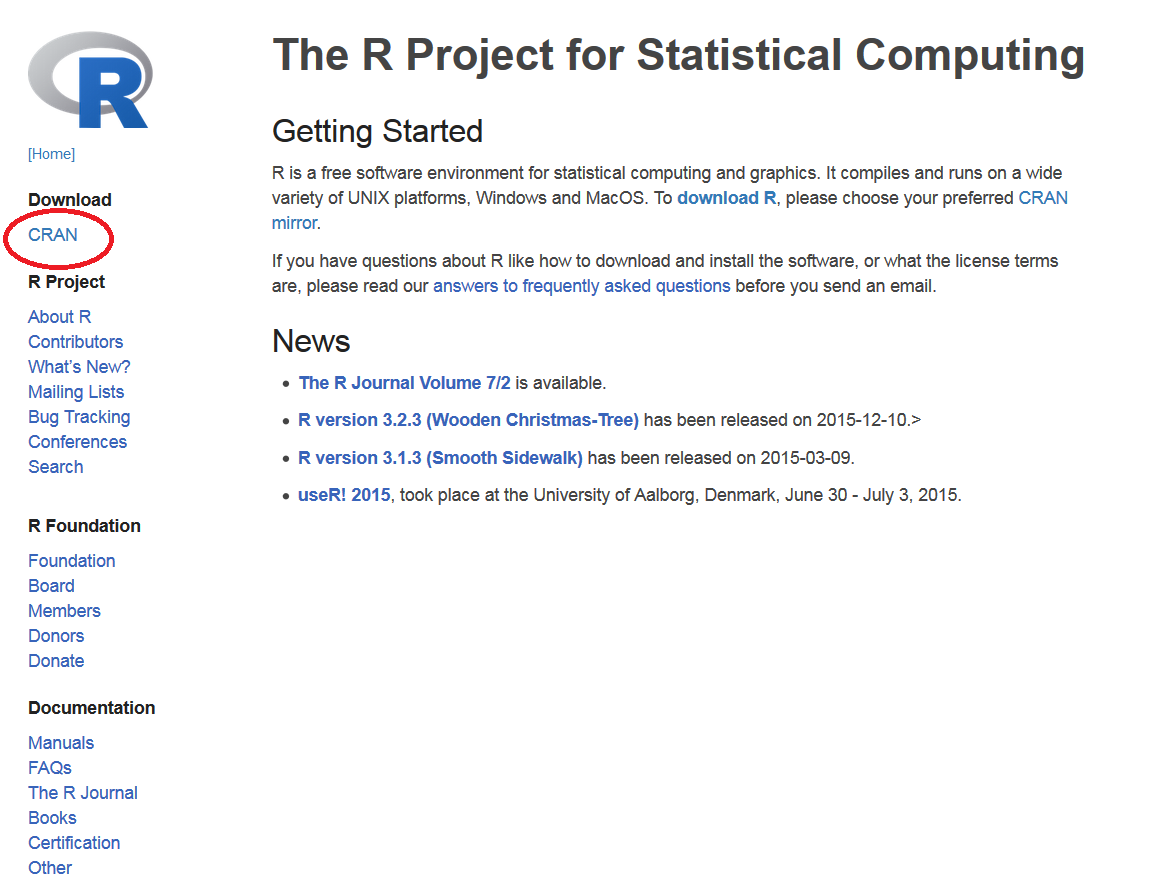
\includegraphics[width=15cm]{R001.png}
\caption{インストール手順1}\label{R001の画像}
\end{figure}
「Japan」の項目を探しその中にある,東京統計数理研究所か山形大学のリンクをクリックする.

\begin{figure}[H]
\centering
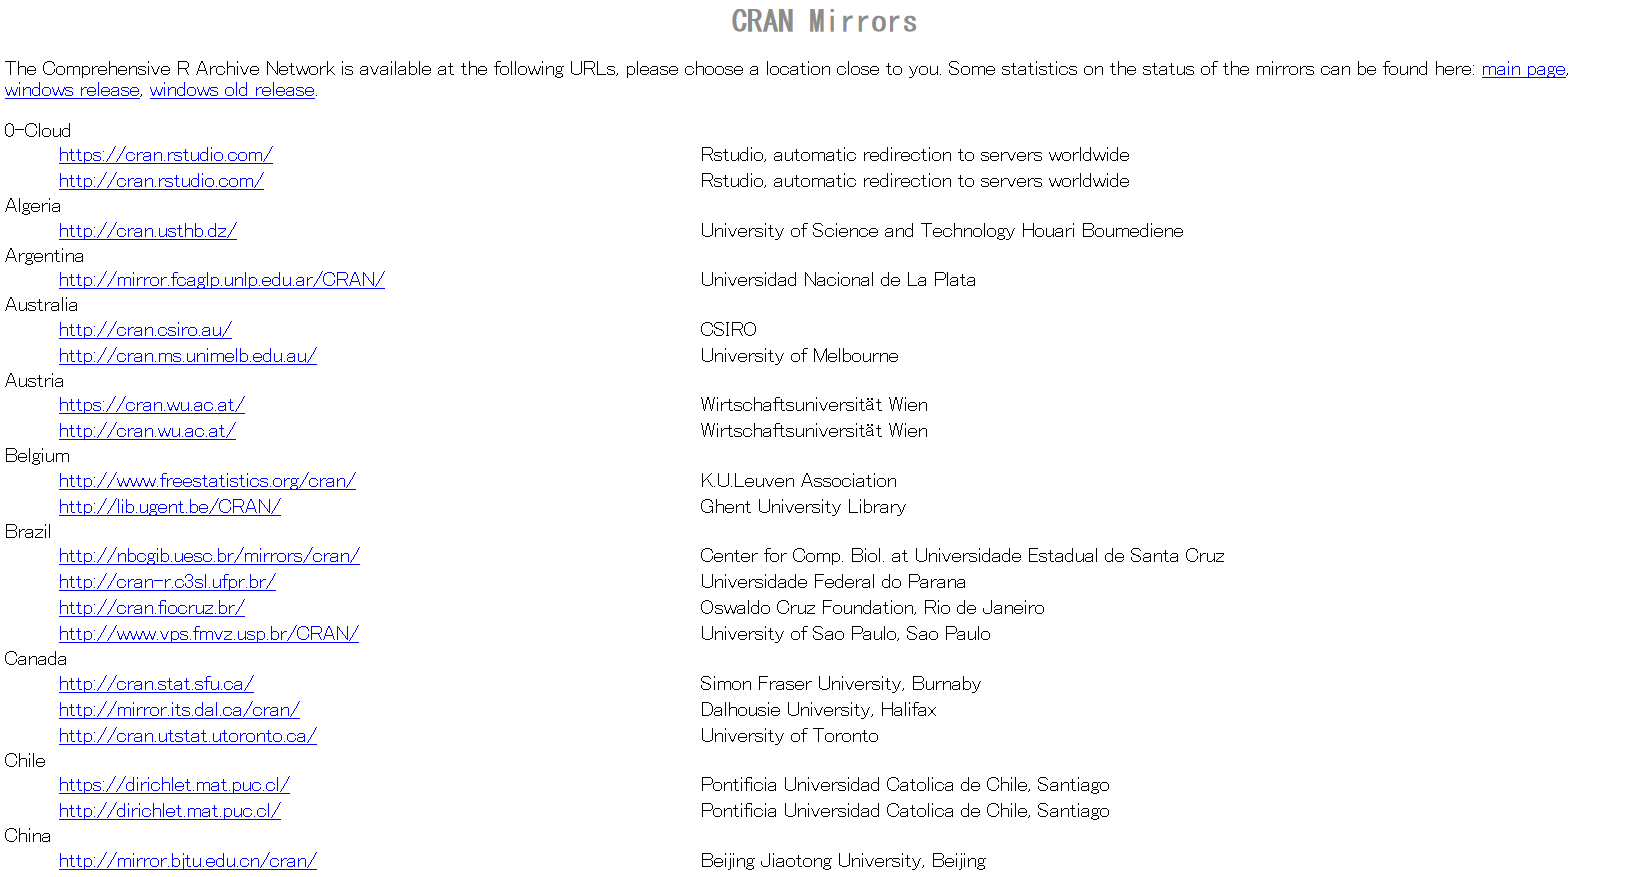
\includegraphics[width=15cm]{R002.png}
\caption{インストール手順2}\label{R002の画像}
\end{figure}

「Download R for Windows」をクリックする.

\begin{figure}[H]
\centering
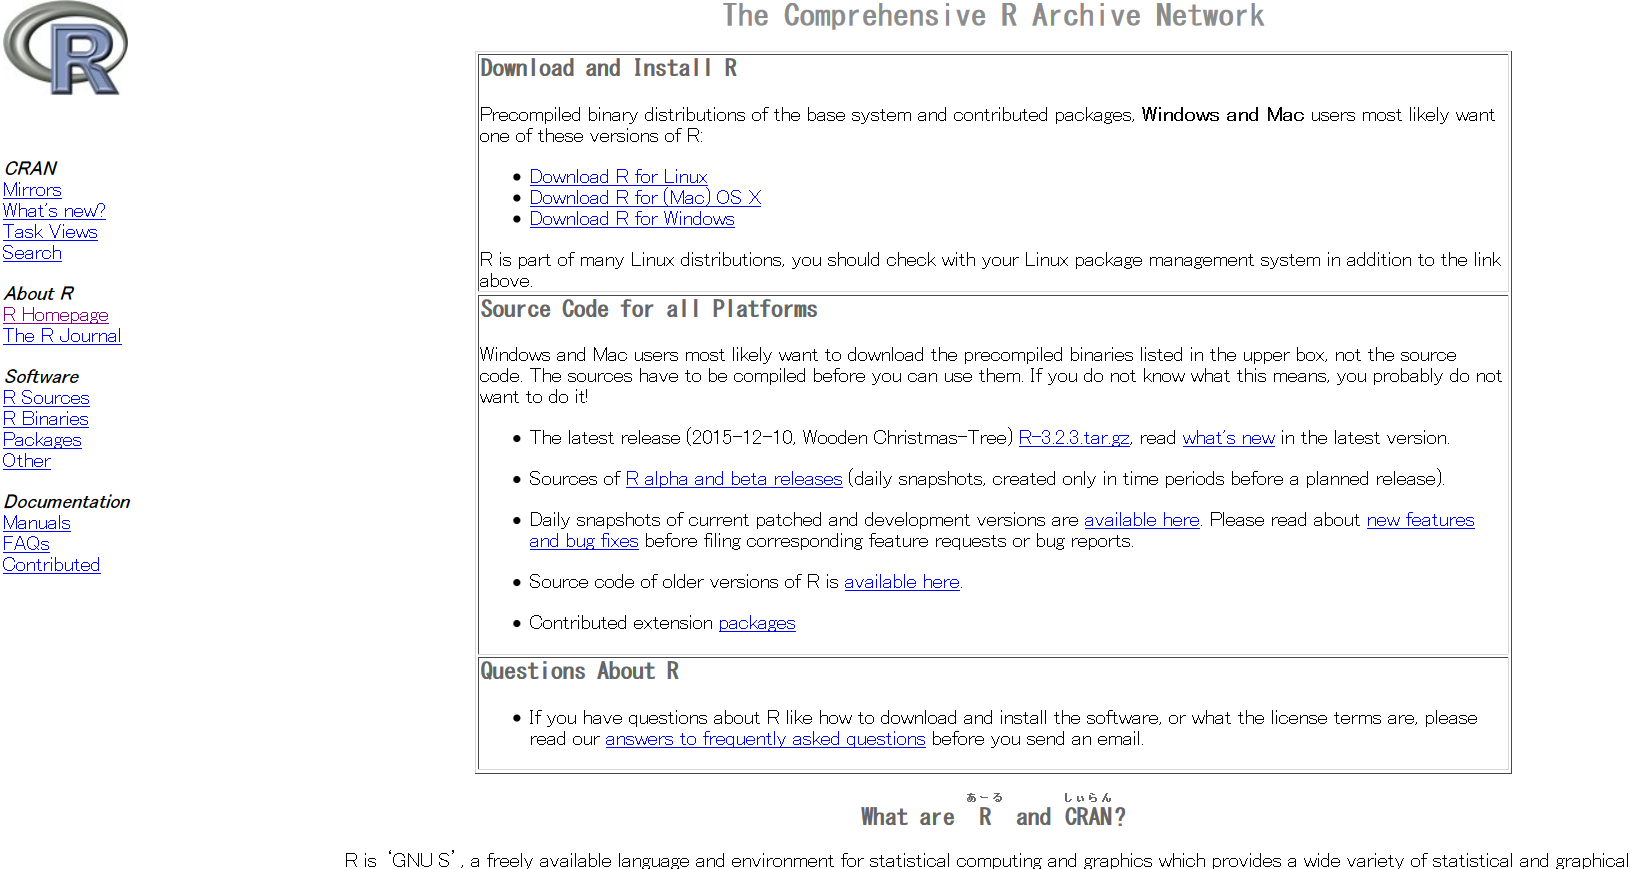
\includegraphics[width=15cm]{R003.png}
\caption{インストール手順3}\label{R003の画像}
\end{figure}
「Download R 3.2.3 for Windows」をクリックするとダウンロードが開始される.


\begin{figure}[H]
\centering
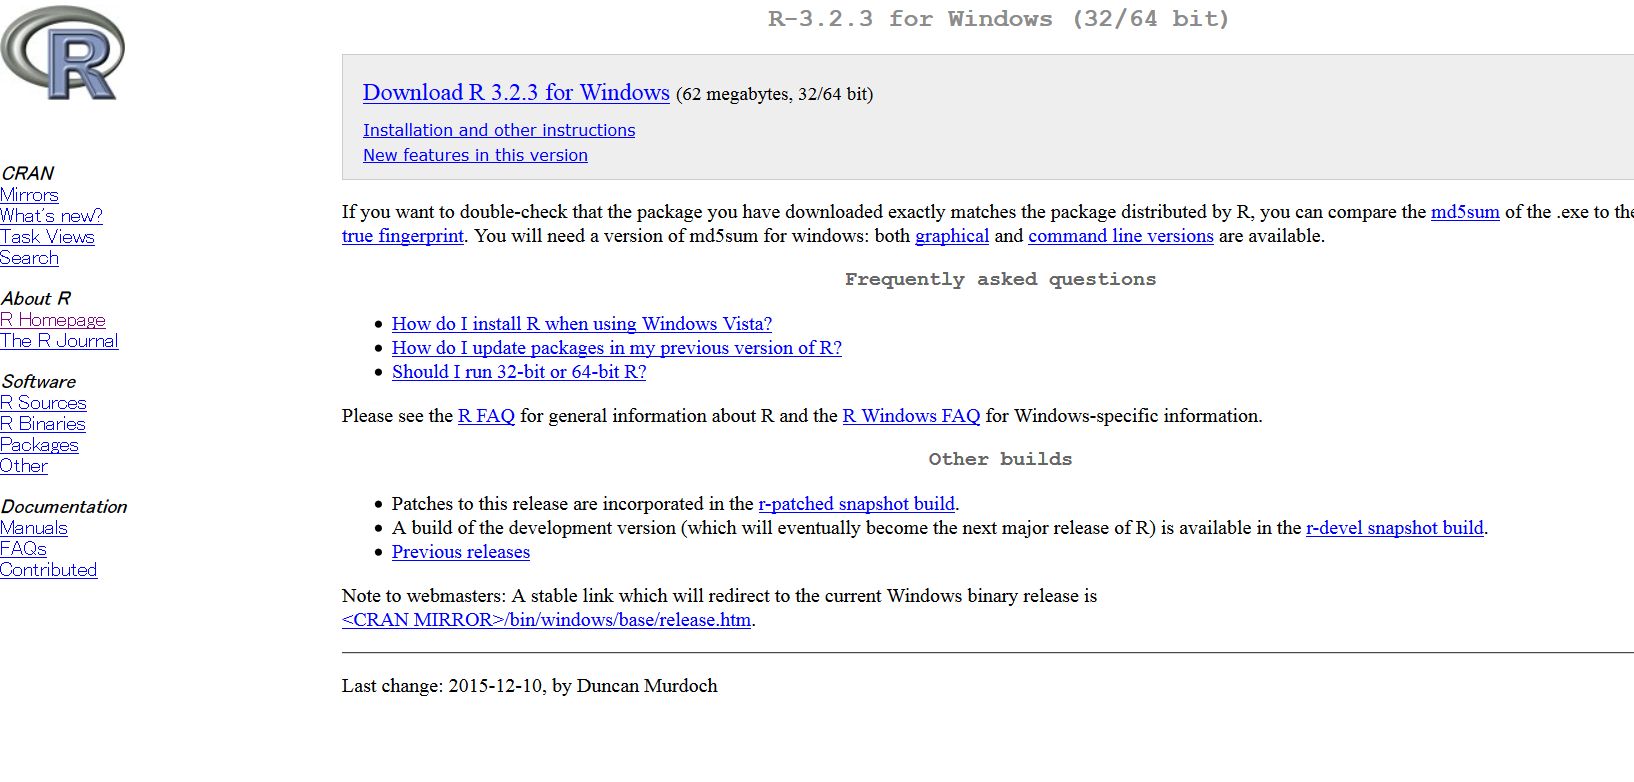
\includegraphics[width=15cm]{R004.png}
\caption{インストール手順4}\label{R004の画像}
\end{figure}

\section{Rの起動と終了}
Rの起動は,インストール時に自動的に作成されるデスクトップ上のRのアイコンをダブルクリックすれば起動する.

\begin{figure}[H]
\centering
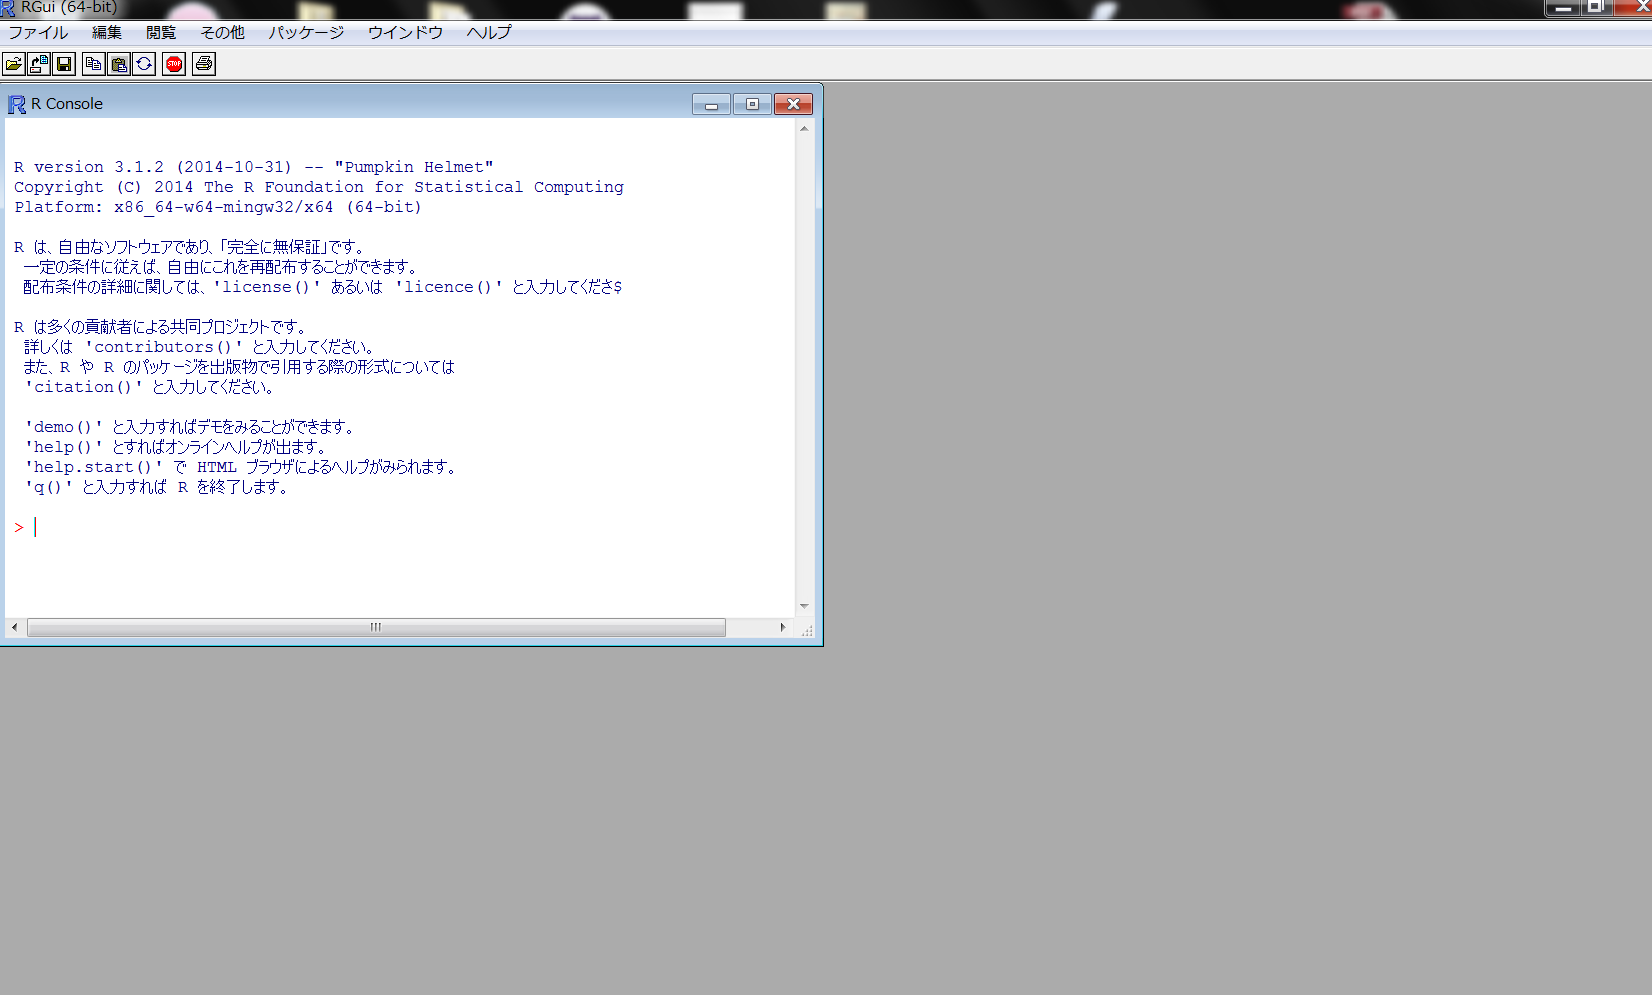
\includegraphics[width=15cm]{R005.png}
\caption{起動画面}\label{R005の画像}
\end{figure}



\chapter{結果,考察}

\section{本章の構成}
本章では第2章で記述した手法を用いて,集めたデータを解析した結果とその考察を記す.

\section{Rを用いた重回帰分析の方法}
第5章で集めてきたデータをRを用いて重回帰分析する方法を記す.
まず,集めたデータをエクセルに保存する.普通に保存するだけではRにエクセルのデータを読み込ませることができないため,保存をする名前をつけた後,「ファイルの種類(T)」から「CSVカンマ区切り」を選択し,保存する.

\begin{figure}[H]
\centering
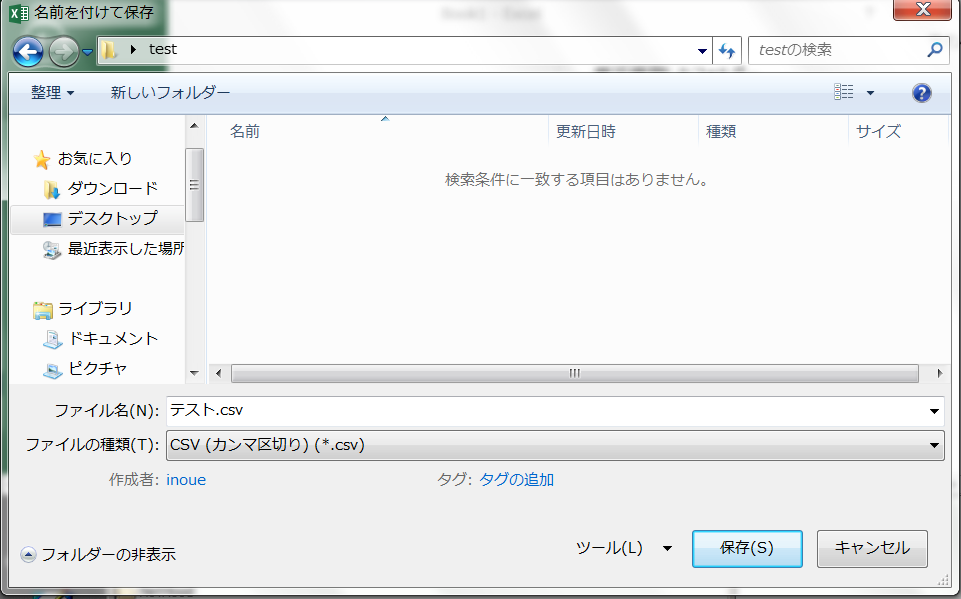
\includegraphics[width=15cm]{kekka001.png}
\caption{保存方法}\label{エクセルの保存方法}
\end{figure}

その後,Rを起動してディレクトリを指定し,ファイルを読み込む.

\begin{figure}[H]
\centering
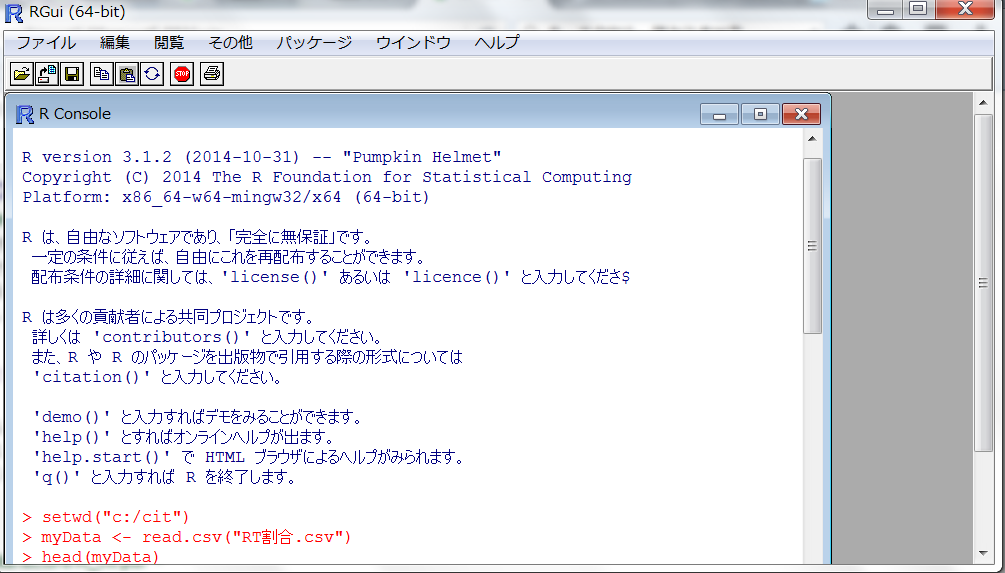
\includegraphics[width=15cm]{kekka002.png}
\caption{Rの画面1}\label{Rの画面1}
\end{figure}

その後重回帰分析をする.

\begin{figure}[H]
\centering
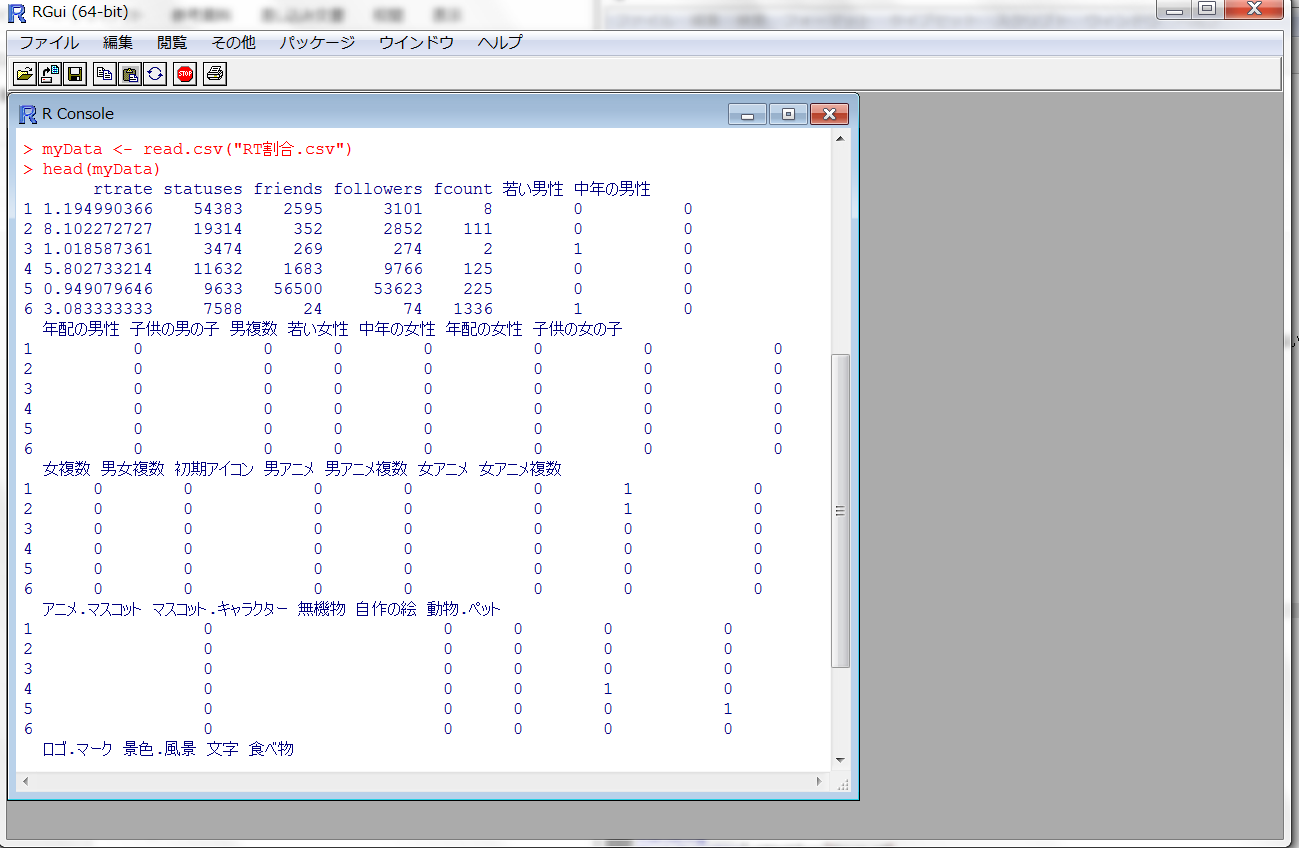
\includegraphics[width=15cm]{kekka003.png}
\caption{Rの画面2}\label{Rの画面1}
\end{figure}


\section{分析結果}

説明変数は,自分で設定したタグ付けしたデータ,目的変数をリツイート数/フォロワー数で重回帰分析した結果が以下である.

\begin{figure}[H]
\centering
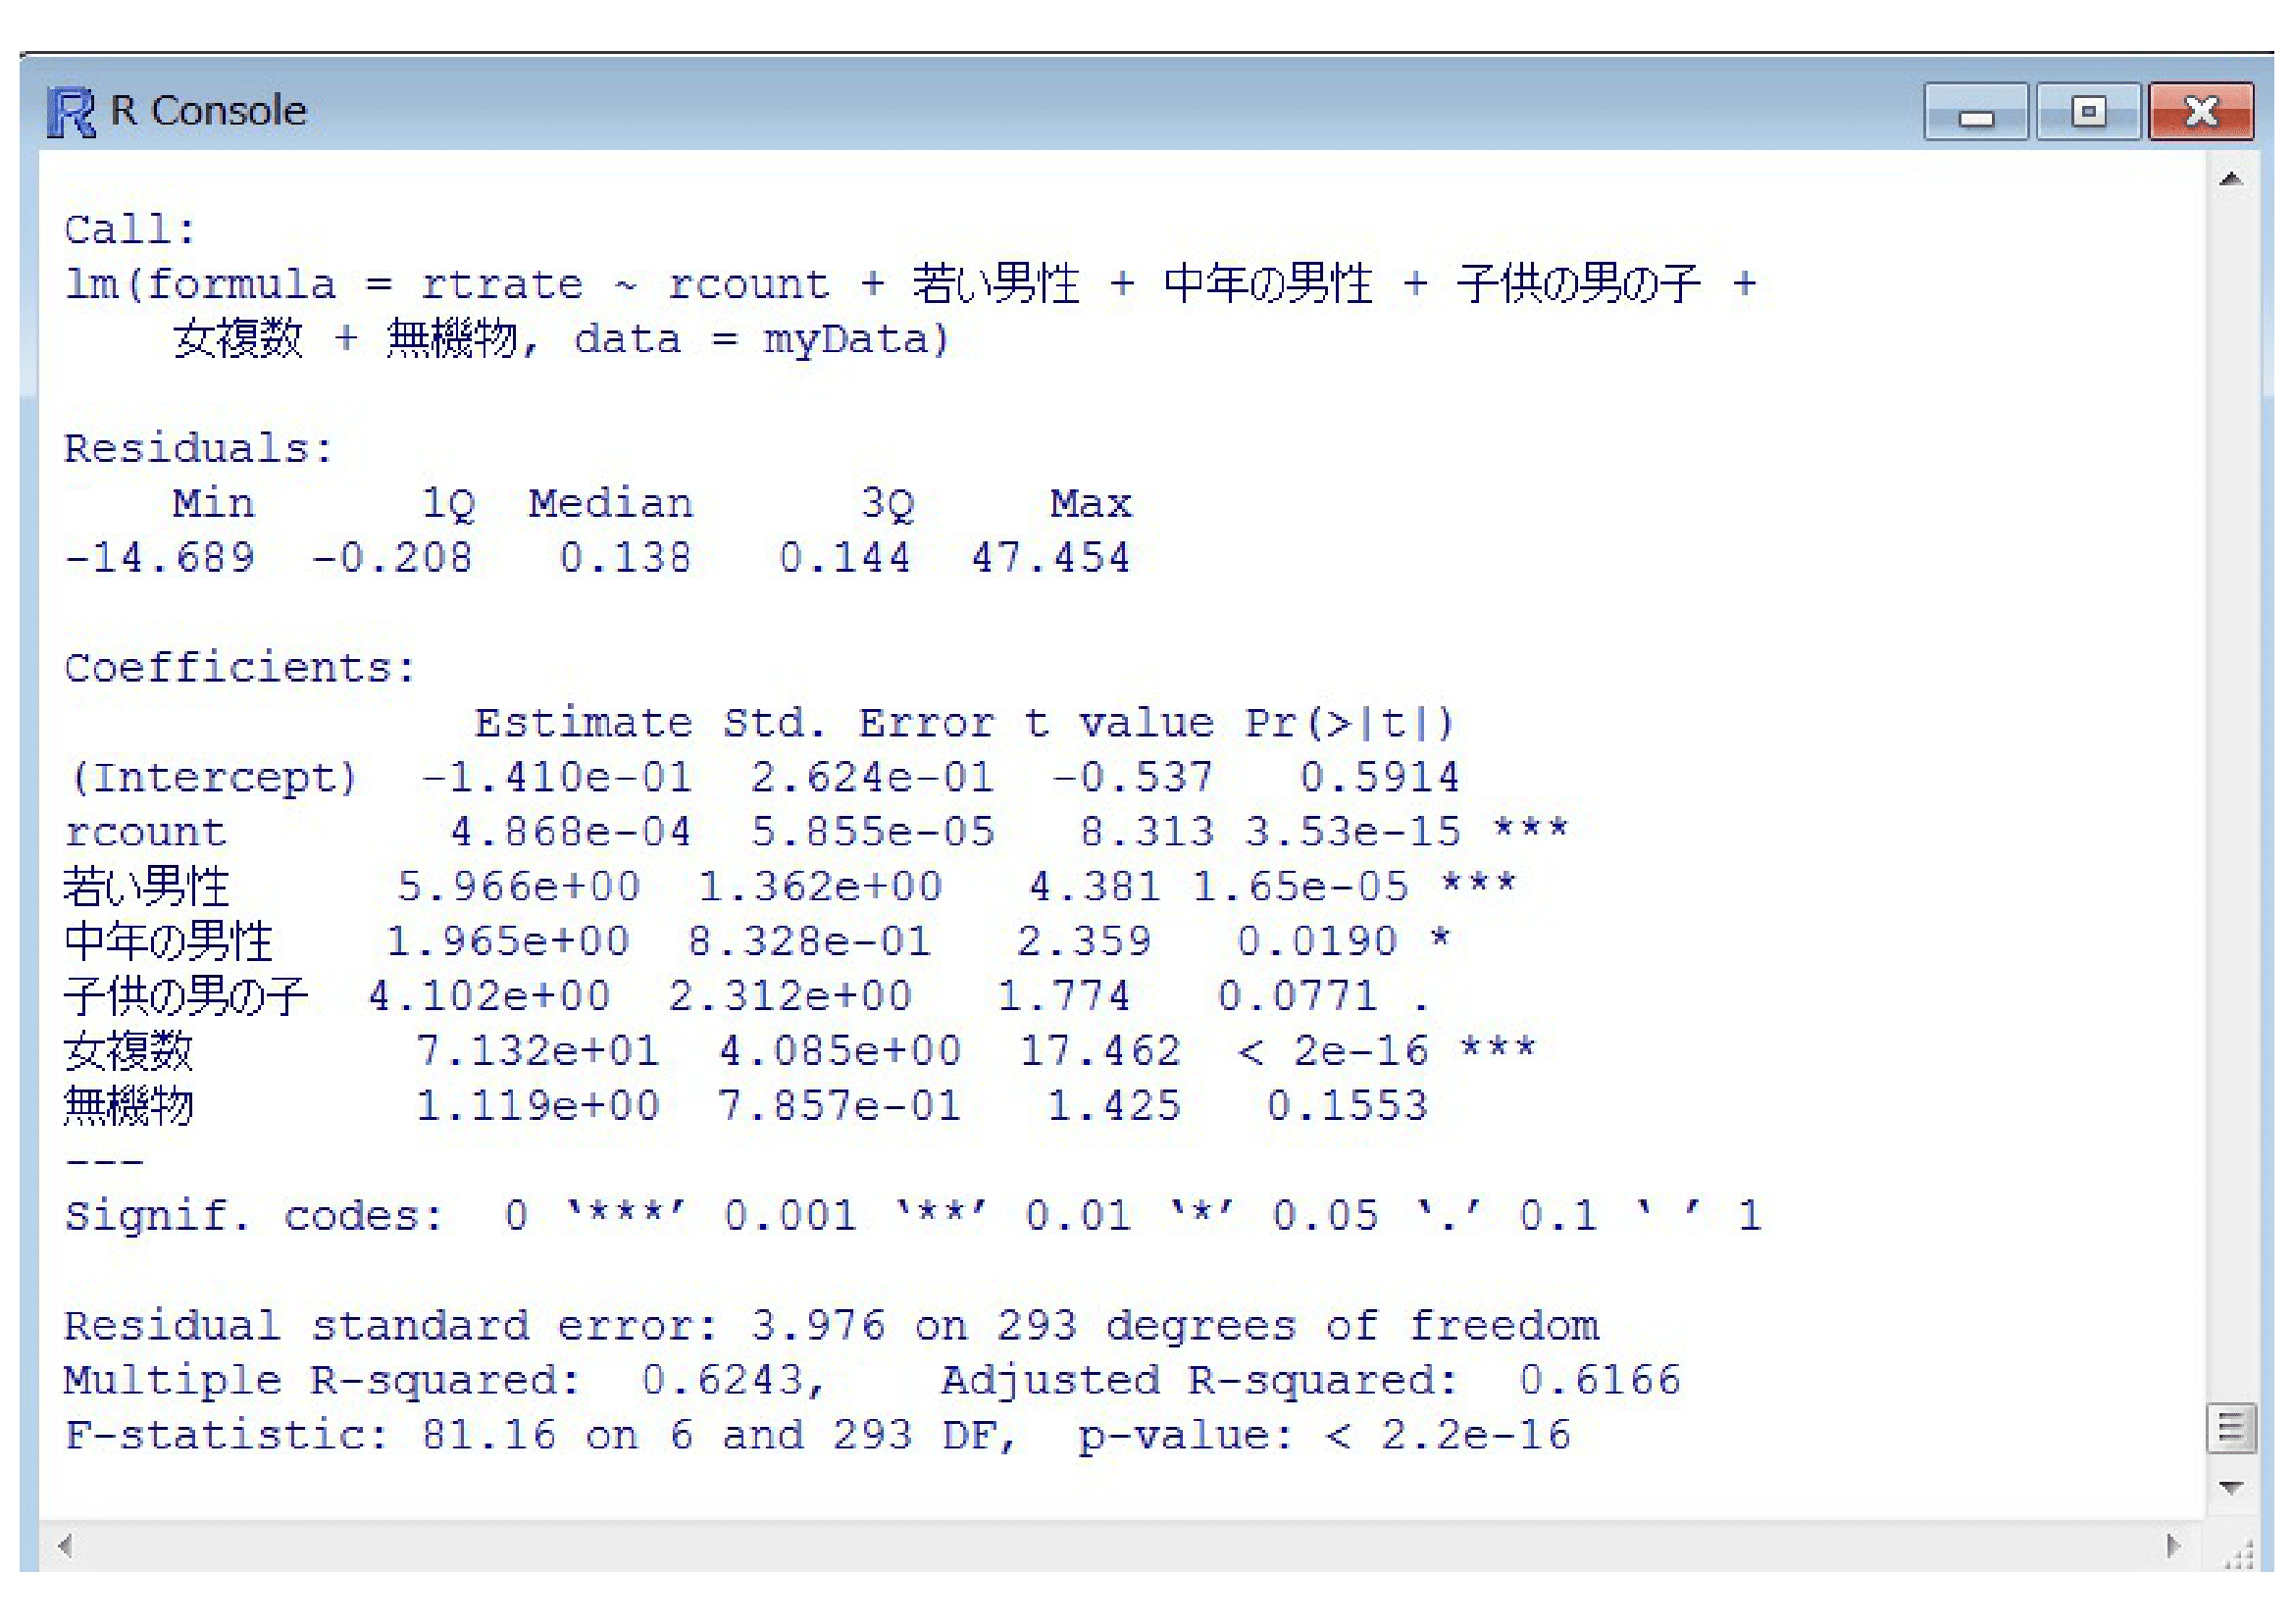
\includegraphics[width=15cm]{kekka004.png}
\caption{分析結果}\label{分析結果}
\end{figure}

若い男性,中年の男性,子供の男の子,女複数,無機物の順番でリツイートされる割合が高い結果が出た.

\section{考察}

以上の結果から全体的に男性のほうがリツイートされる割合が高いということから,ユーザプロフィールのアイコンは拡散力に多少ながら影響があるのではないだろうか.若い男性は新しいブームや流行に追いつきすぐにTwitterに公開しているからではないだろうか,中年の男性は有識人などが多く,社会に対しての問題定義が話題となり拡散力があるのではないだろうかと考えた.


\chapter{結論}

本研究ではTwitterでのアイコンが拡散力に影響するかどうかを見出すことができた.アイコンの画像の種類をタグで分ける際,画像認識サービスも使用したが精度があまりよくなく,研究では使用できなかったため,手作業で分けたため,主観が少し入ってしまった.その点は関しては今後の改善の余地があると言えるだろう.

参考文献は文献ファイル(この文書では\verb|biblio.bib|)に記述し,\verb|\cite|で参照する.例:データベースのための問い合わせ言語SQLで数独を解く方法が提案されている\cite{yabuki2011}.このように参照すると,参考文献リストに自動的に登録される.文献の種類には,雑誌論文\cite{yabuki2011}や会議録論文\cite{yabuki2013},卒業論文\cite{kubo2014},書籍\cite{okumura2013},ウェブサイト\cite{self}などがある.文献の種類によって必要な項目が異なるため,\verb|biblio.bib|を見て確認すること.

\bibliographystyle{junsrt}
\bibliography{biblio}%「biblio.bib」というファイルが必要.

\end{document}